\documentclass{article}
\usepackage[utf8]{inputenc}
\usepackage[margin = 0.8in]{geometry}
\usepackage{graphicx}
\usepackage{amsmath, amssymb}
\usepackage{subcaption}
\usepackage{multirow}
\usepackage{mathtools}
\usepackage{float}
\usepackage{pythonhighlight}


\title{Project 4 - Particle Filters}
\author{Keith Chester}

\begin{document}
\maketitle


In this project we are provided with a subset of data (\textbf{studentdata\textit{N}} where \textit{N} is $0$ through $7$). The data is generated by flying a drone on an indoor course. The drone is recorded by a highly accurate motion capture system, which acts as our ground truth. The drone has an IMU (inertial measurement unit, consisting of an accelerometer and a gyroscope for acceleraton and rotational acceleration respectively), and an on board camera looking down. The floor of the course contains printed AprilTags of a set grid placement, allowing us to estimate a drone position from them alone.

The goal of this project is to demonstrate Particles Filters applied to a nonlinear system (our drone) and produce better estimates than determining the position through the camera alone. For this we will utilize the camera to get an estimated position, note the IMU, and attempt to utilize the filter to smooth the movements out to a realistic tracking path for the drone.

\section*{Task 1}

Task 1 starts us off by instructing us to build the particle filter from which the rest of the assignment will experiment with. Our implementation can be found in \textbf{pf.py}, wherein we create a \textit{ParticleFilter} class. The class is customized with the number of desired particles and other parameters such as noise range to be added during our process model. We attempt to, whenever possible, treat all particles and calculations as vectors and do our best to avoid iteration. This is done to optimize performance and minimize time spent in calculation per step.

For our application problem, we work with a 15 state space vector. When created, the particle filter creates a set of particles, consisting of \textit{N} particles, each being a 15 element vector. We focus only on the first 6 elements of the vector, as the first three represent position and the second three represent orientation. The range of the position is set to be between 0 and 3 meters (save the z axis, which is limited to 1.5 meter) due to observation of the data being ran against - it seems the drone never goes beyond these bounds. The orientation is set to limit the drone in yaw, pitch, and roll in the $-\frac{\pi}{2}$ to $\frac{\pi}{2}$ range.

Once we have our initial particles and our initial position read, we begin iterating through a constant loop until we process all of the data. We calculate the $\Delta t$ since our last read, and run the predict step on every particle.

The predict step attempts to solve xdot, which we know to be:

\begin{equation}
    \dot{x} = \begin{bmatrix}
        \dot{p}            \\
        G(q)^{-1} \omega_w \\
        g + R(q) \omega_a  \\
        n_g                \\
        n_a
    \end{bmatrix}
\end{equation}

...wherein $\dot{p}$ is the derivative of our position, $G(q)$ is the rotation matrix from the world frame to the drone frame, $\omega_w$ is the force vector, $R(q)$ is the rotation matrix from the drone frame to the world frame, $\omega_a$ is the acceleration vector (gravity is negative due to frame orientation), $n_g$ is the bias from the gyroscope, and $n_a$ is the bias from the accelerometer.

We then apply the $\Delta t$ to the $\dot{x}$ vector to get our new position:

\begin{equation}
    x_{t+1} = x_t + \dot{x} \Delta t
\end{equation}

When we do this calculation, we also generate noise based on a configurable hyperparameter for our class. We experimented with how to add this noise, landing on three possible routes:

\begin{itemize}
    \item Add the noise directly to $\omega_w$ and $\omega_a$ before applying the $\Delta t$
    \item Add the noise universally across the $\dot{x}$ vector prior to applying the $\Delta t$
    \item Add the noise universally across the new $x$ vector after adding $\dot{x}$.
\end{itemize}

Ultimately we decided to add the noise to the $\omega_w$ and $\omega_a$ vectors before applying the $\Delta t$. In a future section of this paper we will discuss how we narrowed down what noise values to use.

After the predict section, we estimate the pose of the drone from the image data through the use of the \text{solvePnP} function. We take this measurement and perform the update step, wherein we apply the diagonal of our calculated covariance matrix to our measured state. This matrix was calculated in a prior assignment, and is listed below as $C_{measurement}$:

\begin{equation}
    \begin{bmatrix}
        7.09701409e-03 & 2.66809900e-05  & 1.73906943e-03  & 4.49014777e-04  & 3.66195490e-03  & 8.76154421e-04  \\
        2.66809900e-05 & 4.70388499e-03  & -1.33432420e-03 & -3.46505064e-03 & 1.07454548e-03  & -1.69184839e-04 \\
        1.73906943e-03 & -1.33432420e-03 & 9.00885499e-03  & 1.80220246e-03  & 3.27846190e-03  & -1.11786368e-03 \\
        4.49014777e-04 & -3.46505064e-03 & 1.80220246e-03  & 5.27060654e-03  & 1.01361187e-03  & -5.86487142e-04 \\
        3.66195490e-03 & 1.07454548e-03  & 3.27846190e-03  & 1.01361187e-03  & 7.24994152e-03  & -1.36454993e-03 \\
        8.76154421e-04 & -1.69184839e-04 & -1.11786368e-03 & -5.86487142e-04 & -1.36454993e-03 & 1.21162646e-03  \\
    \end{bmatrix}
\end{equation}

our update step modifies the estimated state $x_t$ to $x_u$ via:

\begin{equation}
    x_u = I_{6x6} x_t + C_{measurement}
\end{equation}

We then calculate the weights of the existing particles based on this measured prediction. Initially, the weights are set to $\frac{1}{N}$, but each future step they are:

\begin{equation}
    W_i = \frac{1}{\sqrt{\Sigma (x_i - x_u)^2}}
\end{equation}

We then normalize the weights to ensure they sum to 1, via:

\begin{equation}
    W_i = \frac{W_i}{\Sigma W}
\end{equation}

We then select the estimate from the weights and particles in one of several manners - by the highest weighted particle, the weighted average of all particles, or the flat average of all particles. We explore the performance of each later.

Finally, we resample each particle each step. This works by stochastically selecting a subset of the particles with a higher probability of tossing low weighted particles and keeping high weighted particles.

The process continues until we have created an estimate for each position across the entire dataset.

\subsection*{Noise Hyperparameter Search}

Earlier we mentioned that we experimented with different noise methods; we also experimented with different noise values in order to find the "best performing" across all datasets for a singular generic value. We note that the first dataset, \textit{studentdata0}, exhibited significant "teleportation" at parts due to the camera losing sight of AprilTags, resulting in that dataset performing particularly worse.

To do this, we created \textbf{noise\_tester.py}, which runs the particle filter with a set number of particles ($2000$), but modifies the noise added to $\omega_a$ and $\omega_w$. We ran these values across all datasets, calculating the RMSE and exporting to a CSV file. RMSE is defined as:

\begin{equation}
    e = \sqrt{\frac{\Sigma (x_{true} - x_{est})^2}{N}}
\end{equation}

A quick utilization of a spreadsheet client allowed us to quickly average the RMSE across specific noise combinations. Over time we expanded and then refined the search space of the noise values, finally landing on a set of values that worked across most datasets well, setting them as the defaults in the \textit{ParticleFilter} class.

\subsection*{Dataset Demonstrations}

Below are the results of various datasets and the default values of the particle filter, with 2000 particles:

\begin{figure}[H]
    \centering
    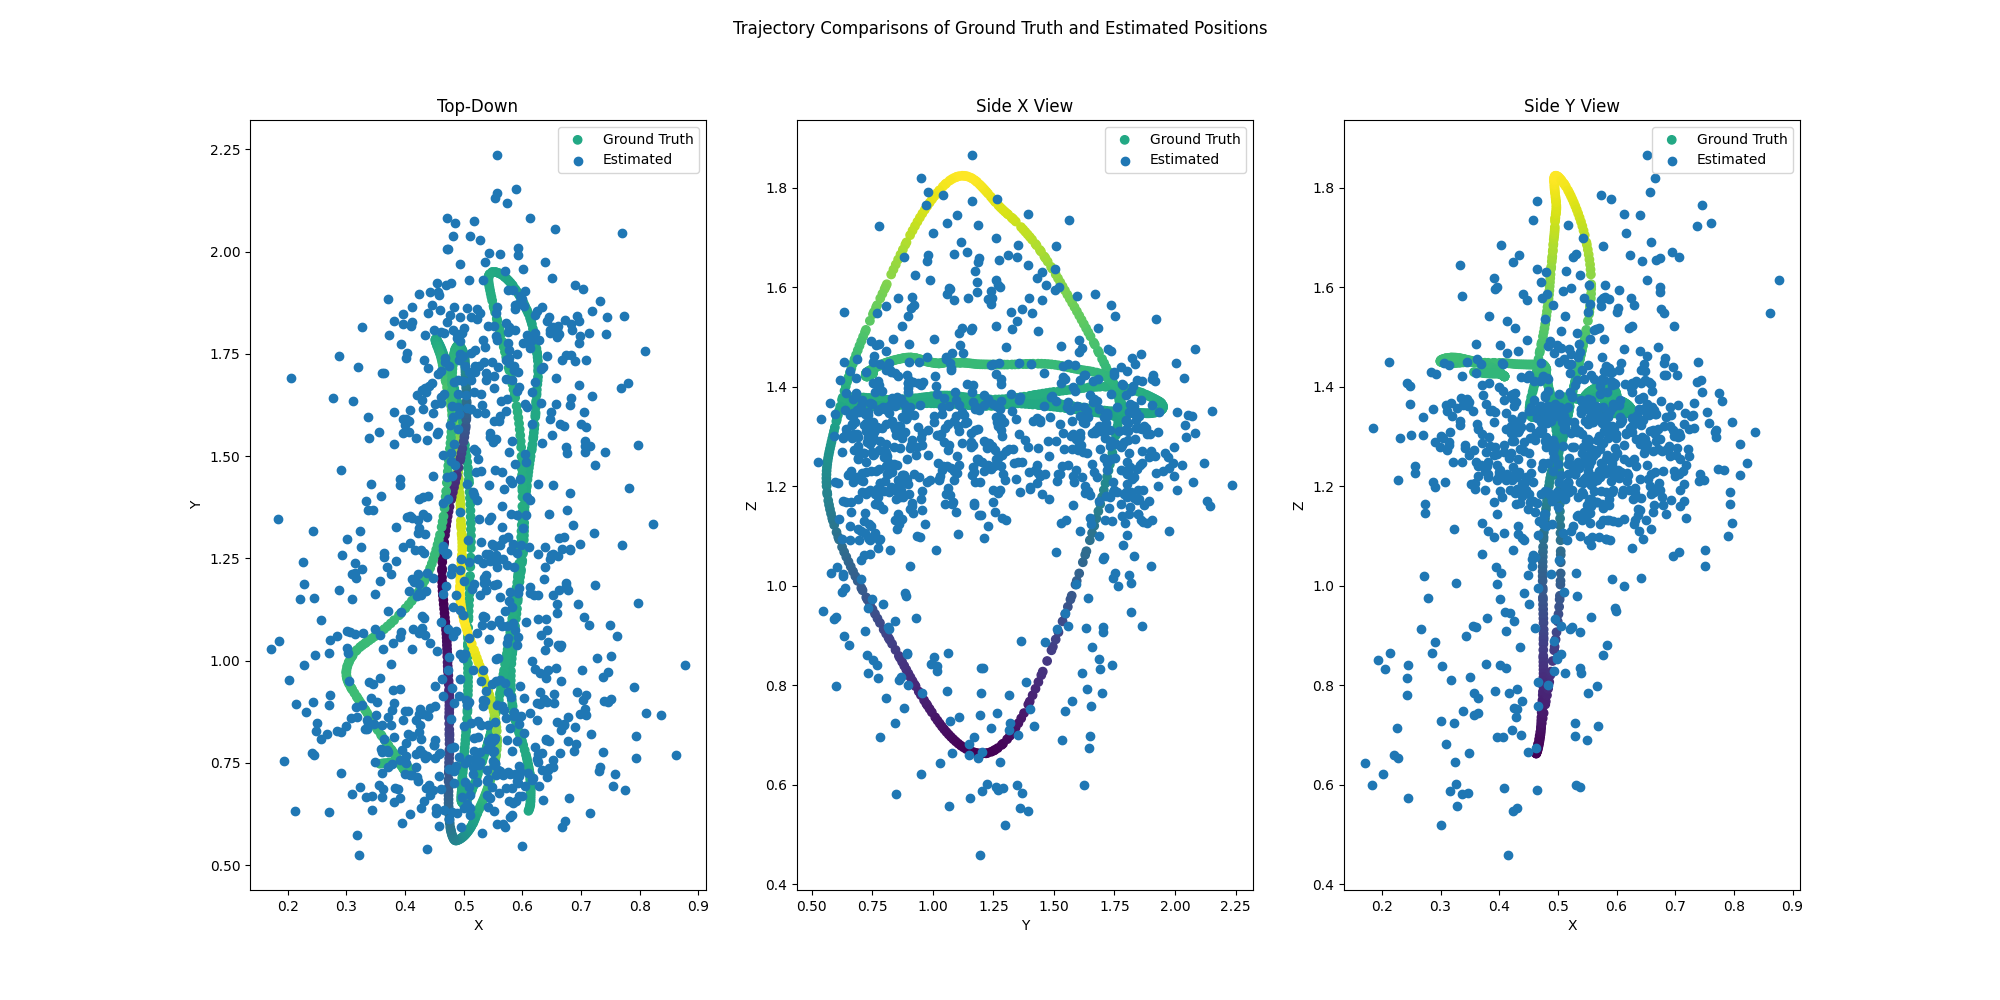
\includegraphics[width=0.8\textwidth]{./imgs/task1/studentdata1_positions.png}
    \caption{Dataset 1 Trajectories}
\end{figure}

\begin{figure}[H]
    \centering
    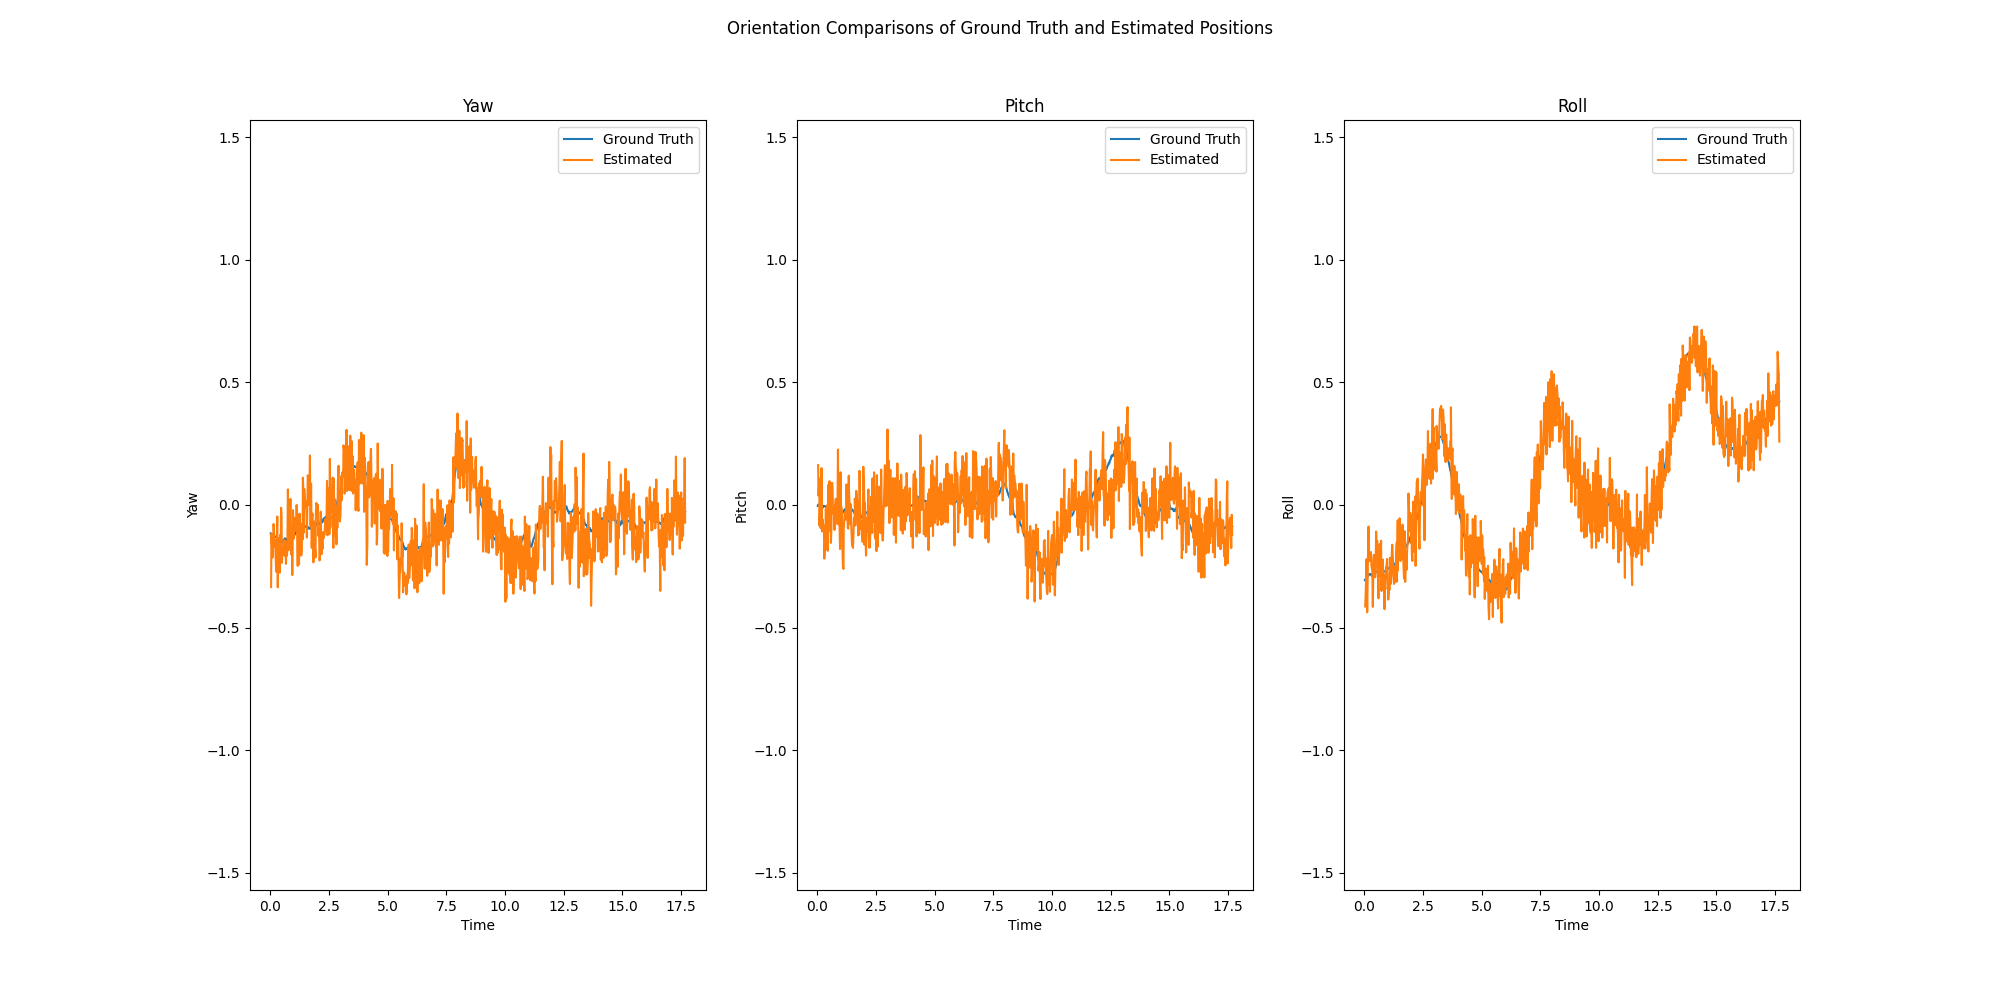
\includegraphics[width=0.8\textwidth]{./imgs/task1/studentdata1_orientations.png}
    \caption{Dataset 1 Orientations}
\end{figure}

\begin{figure}[H]
    \centering
    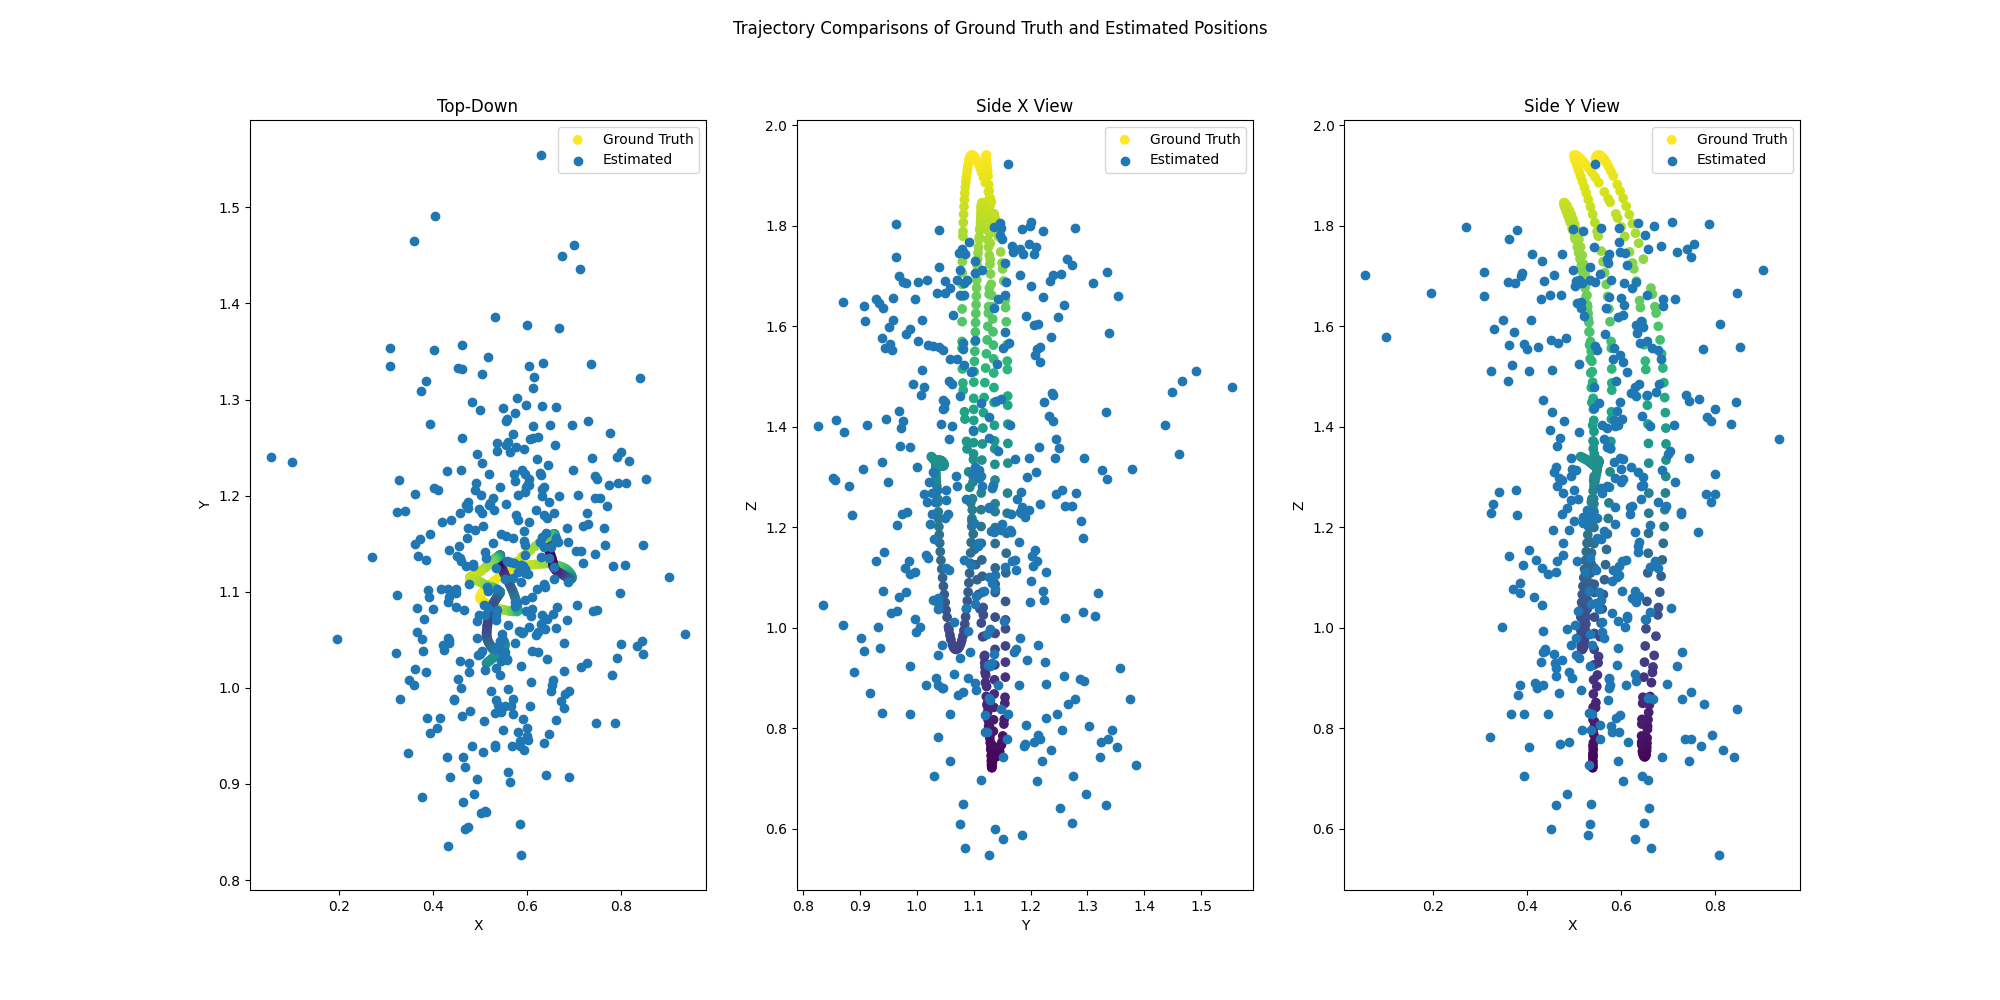
\includegraphics[width=0.8\textwidth]{./imgs/task1/studentdata2_positions.png}
    \caption{Dataset 2 Trajectories}
\end{figure}

\begin{figure}[H]
    \centering
    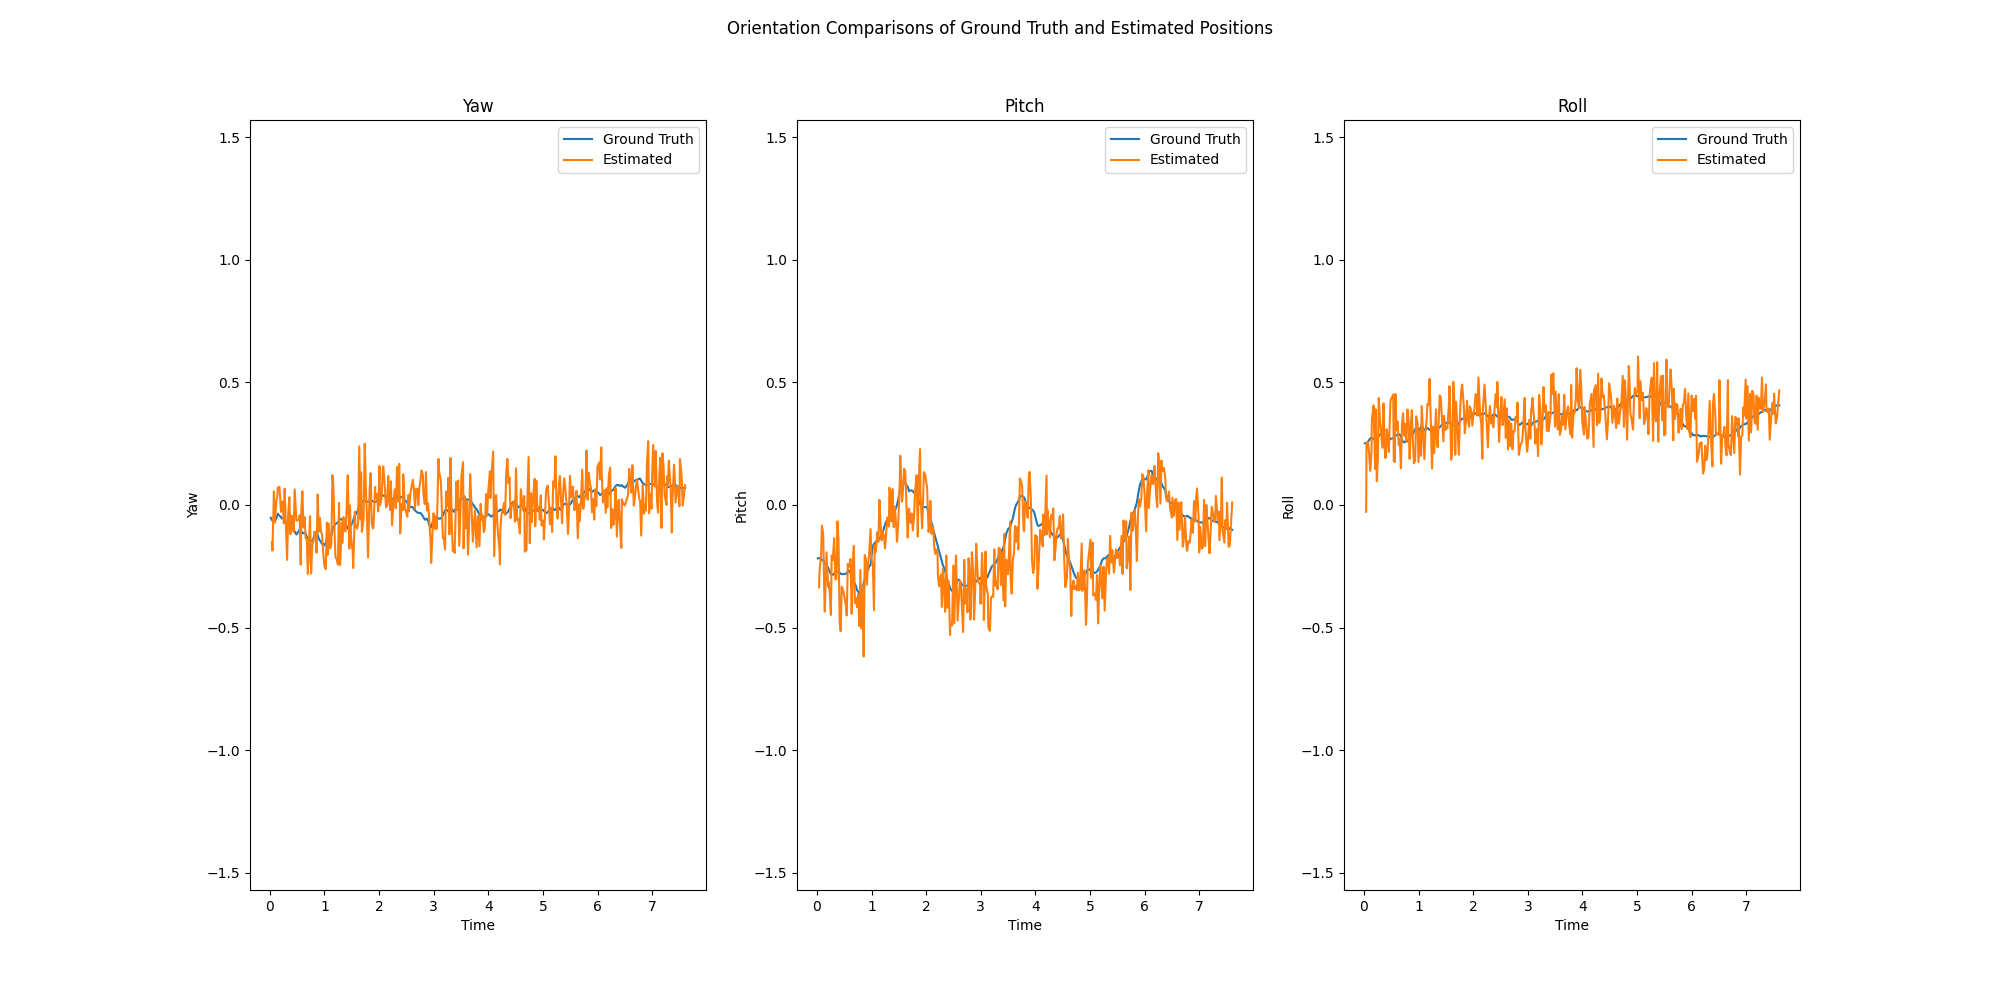
\includegraphics[width=0.8\textwidth]{./imgs/task1/studentdata2_orientations.png}
    \caption{Dataset 2 Orientations}
\end{figure}

\begin{figure}[H]
    \centering
    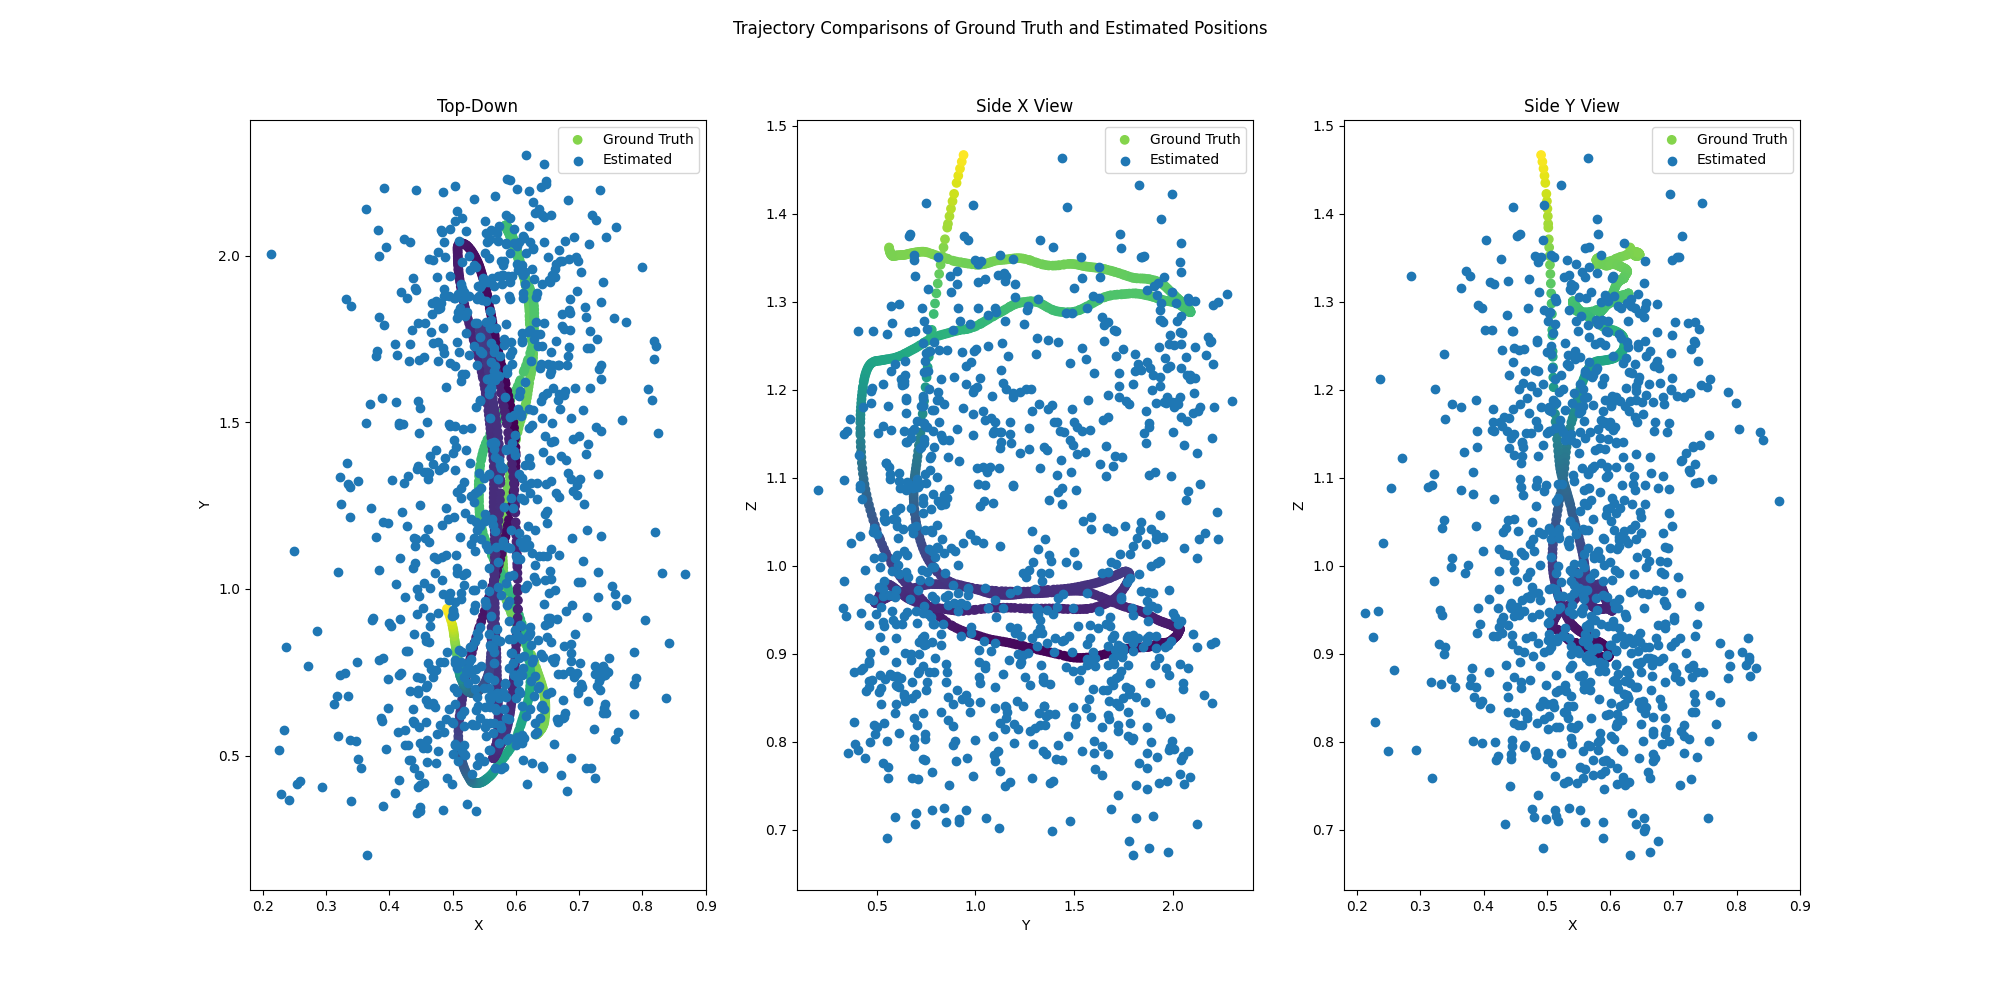
\includegraphics[width=0.8\textwidth]{./imgs/task1/studentdata3_positions.png}
    \caption{Dataset 3 Trajectories}
\end{figure}

\begin{figure}[H]
    \centering
    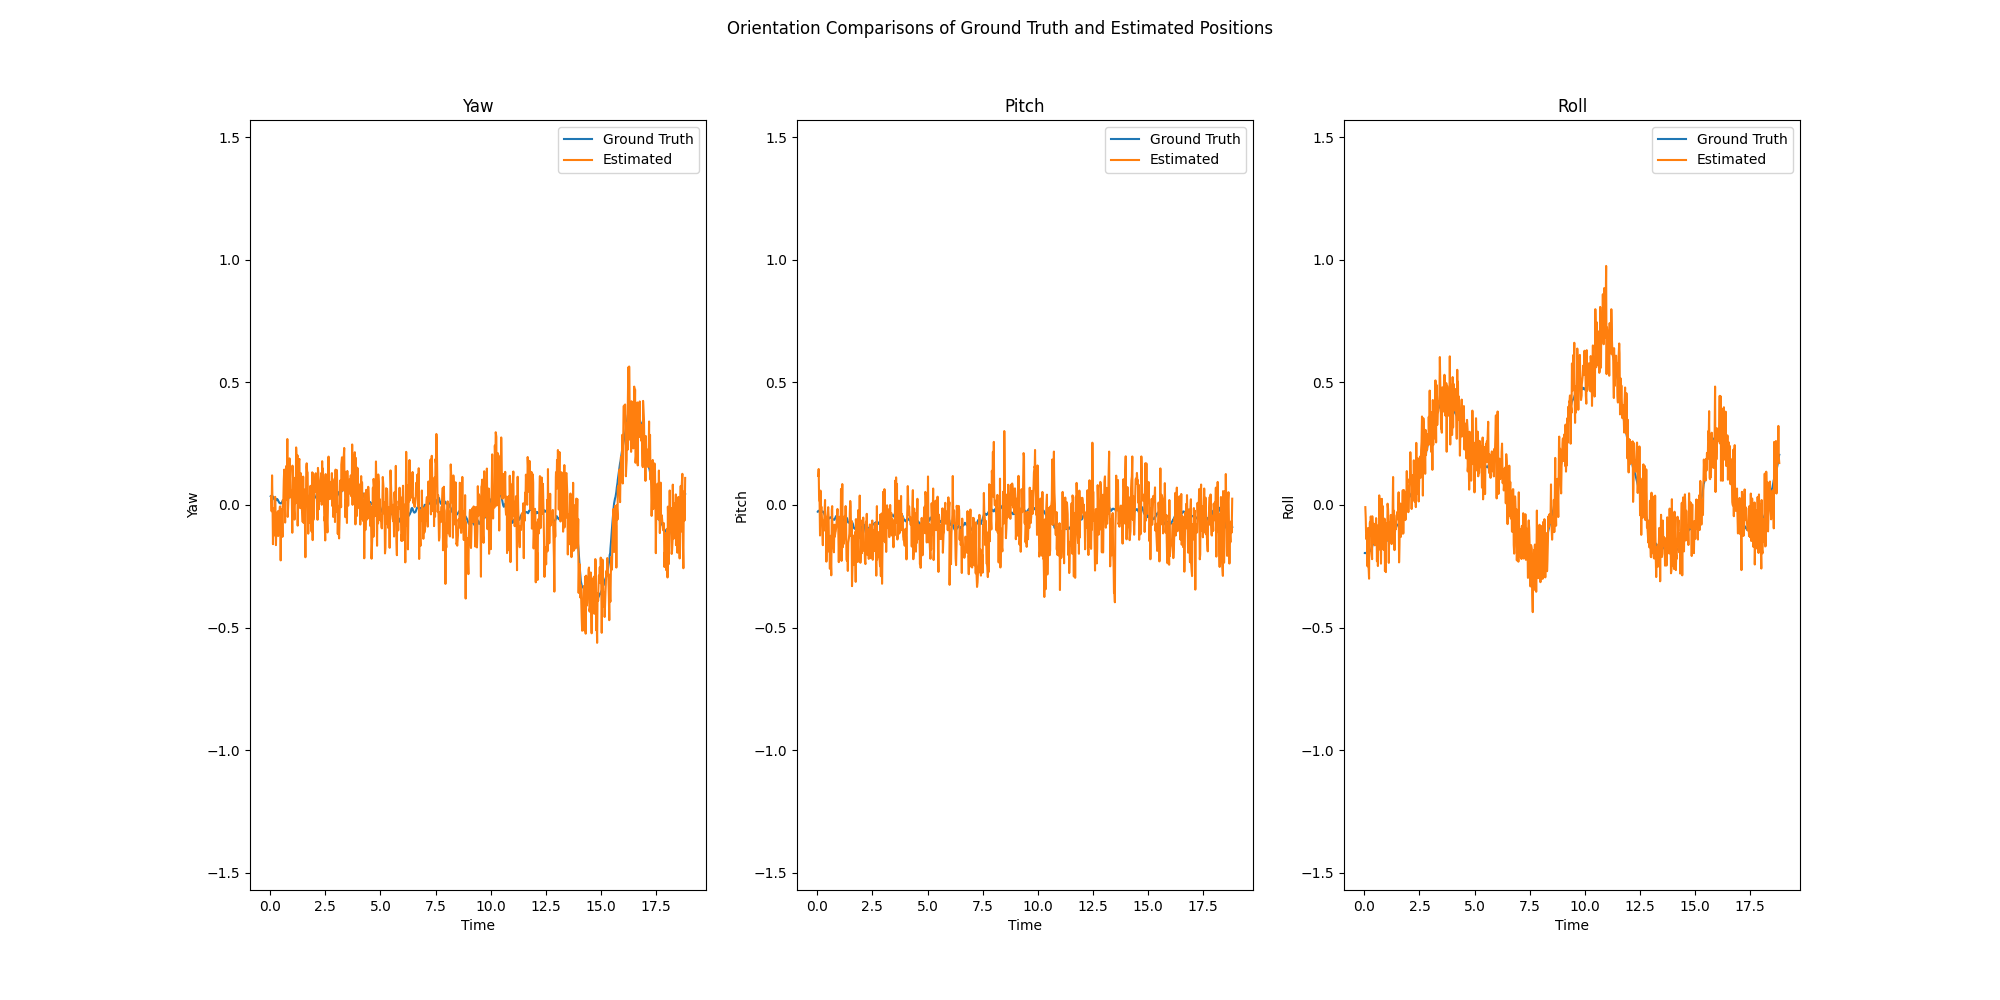
\includegraphics[width=0.8\textwidth]{./imgs/task1/studentdata3_orientations.png}
    \caption{Dataset 3 Orientations}
\end{figure}

\begin{figure}[H]
    \centering
    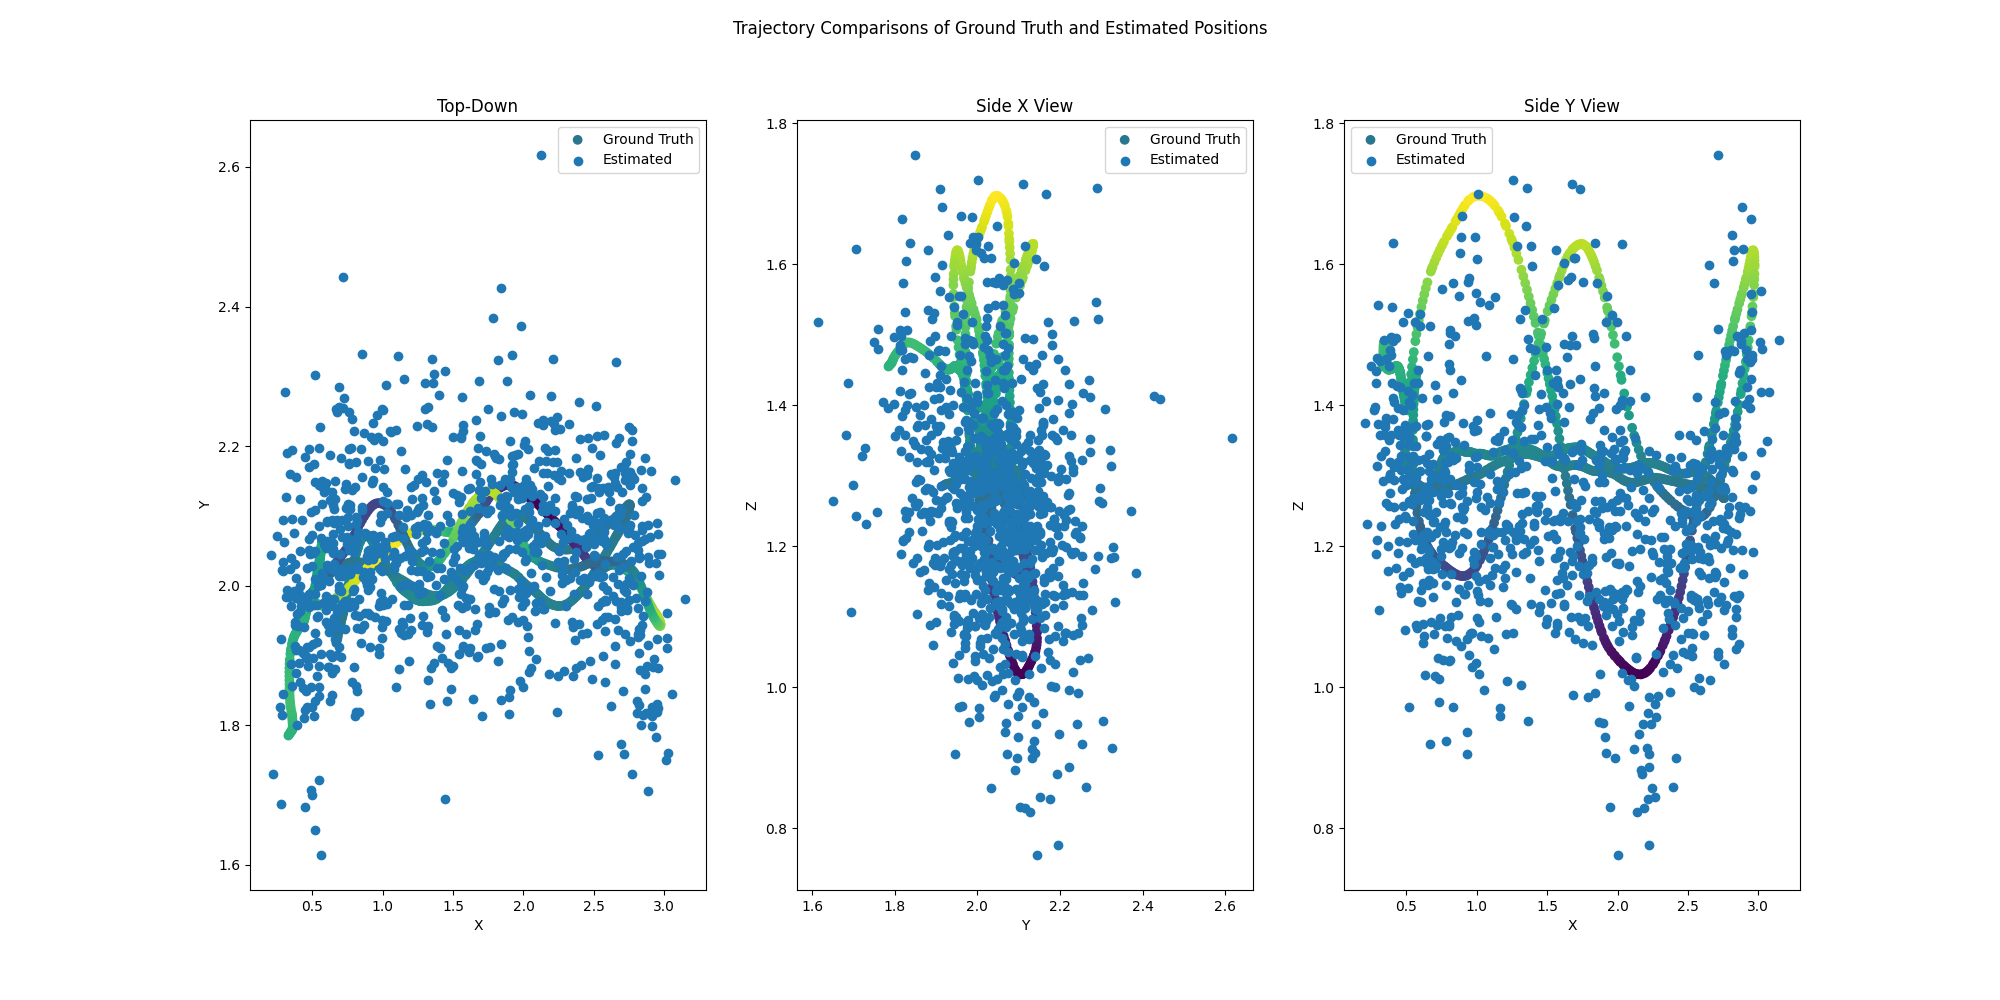
\includegraphics[width=0.8\textwidth]{./imgs/task1/studentdata4_positions.png}
    \caption{Dataset 4 Trajectories}
\end{figure}

\begin{figure}[H]
    \centering
    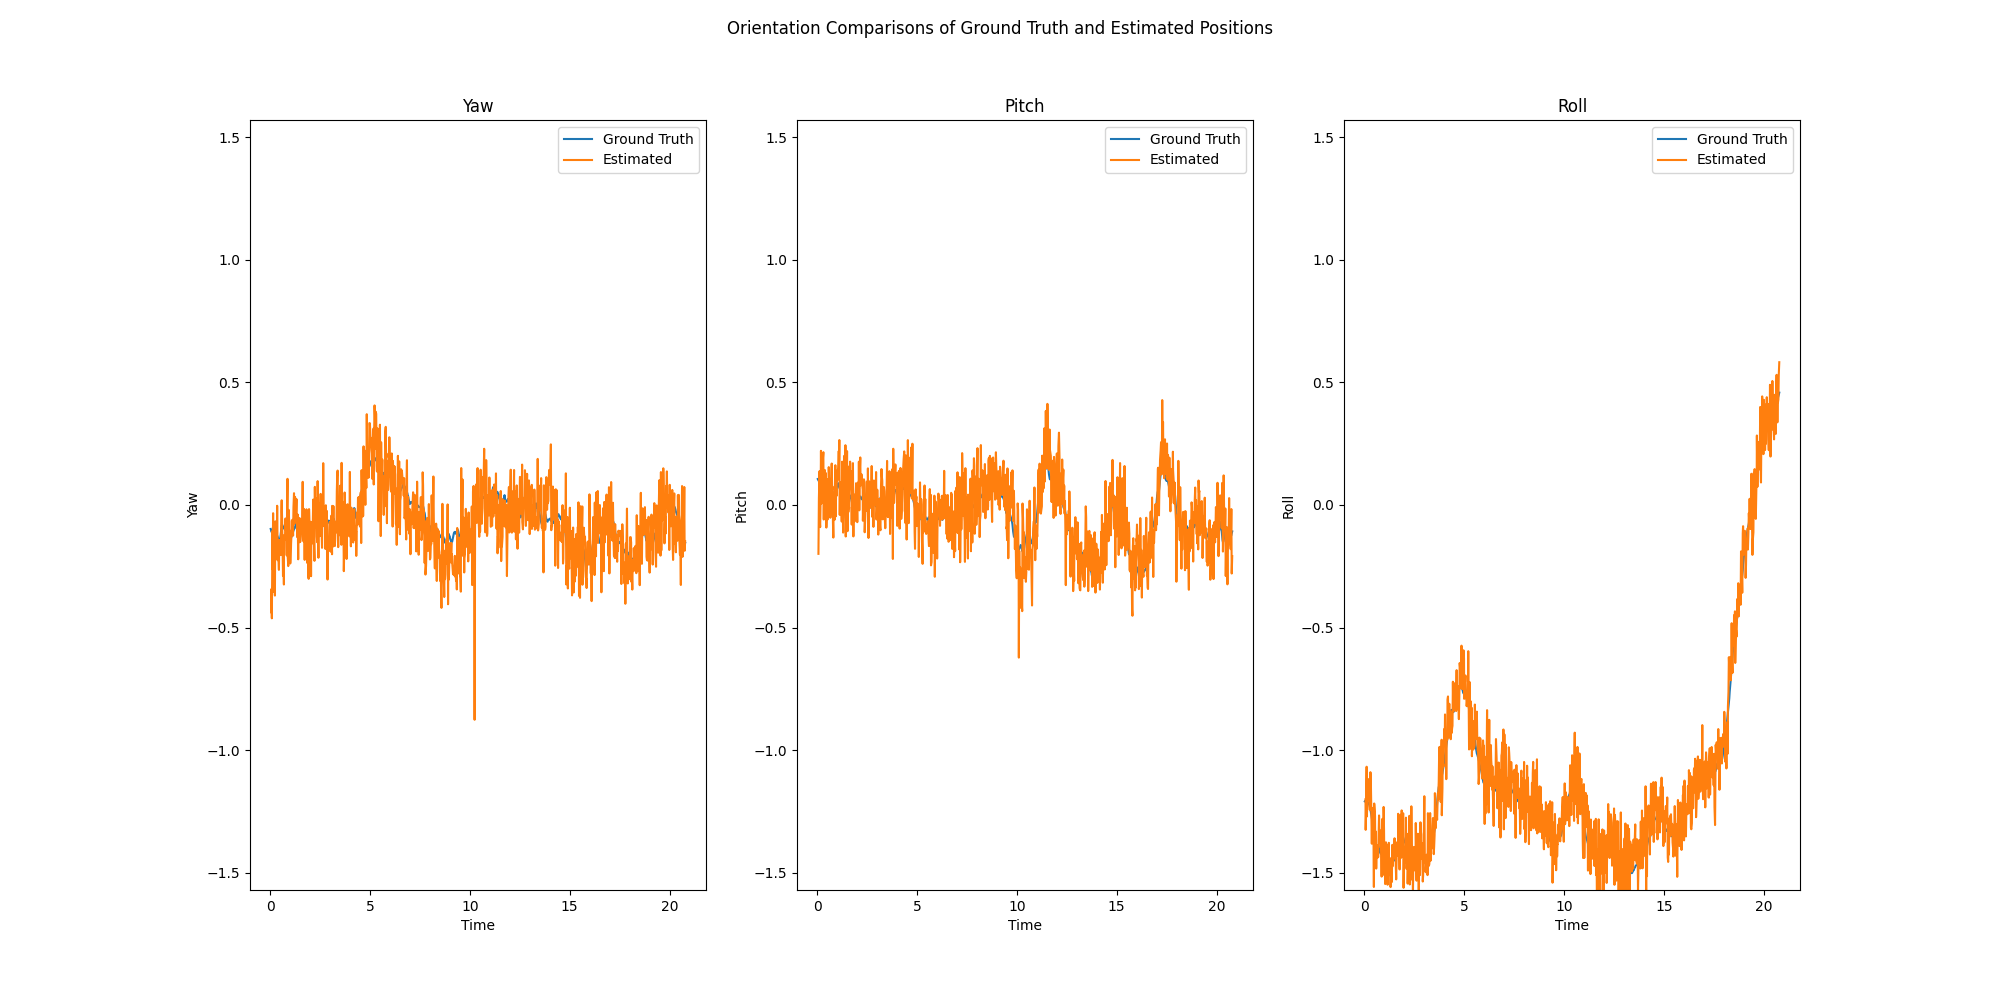
\includegraphics[width=0.8\textwidth]{./imgs/task1/studentdata4_orientations.png}
    \caption{Dataset 4 Orientations}
\end{figure}

\begin{figure}[H]
    \centering
    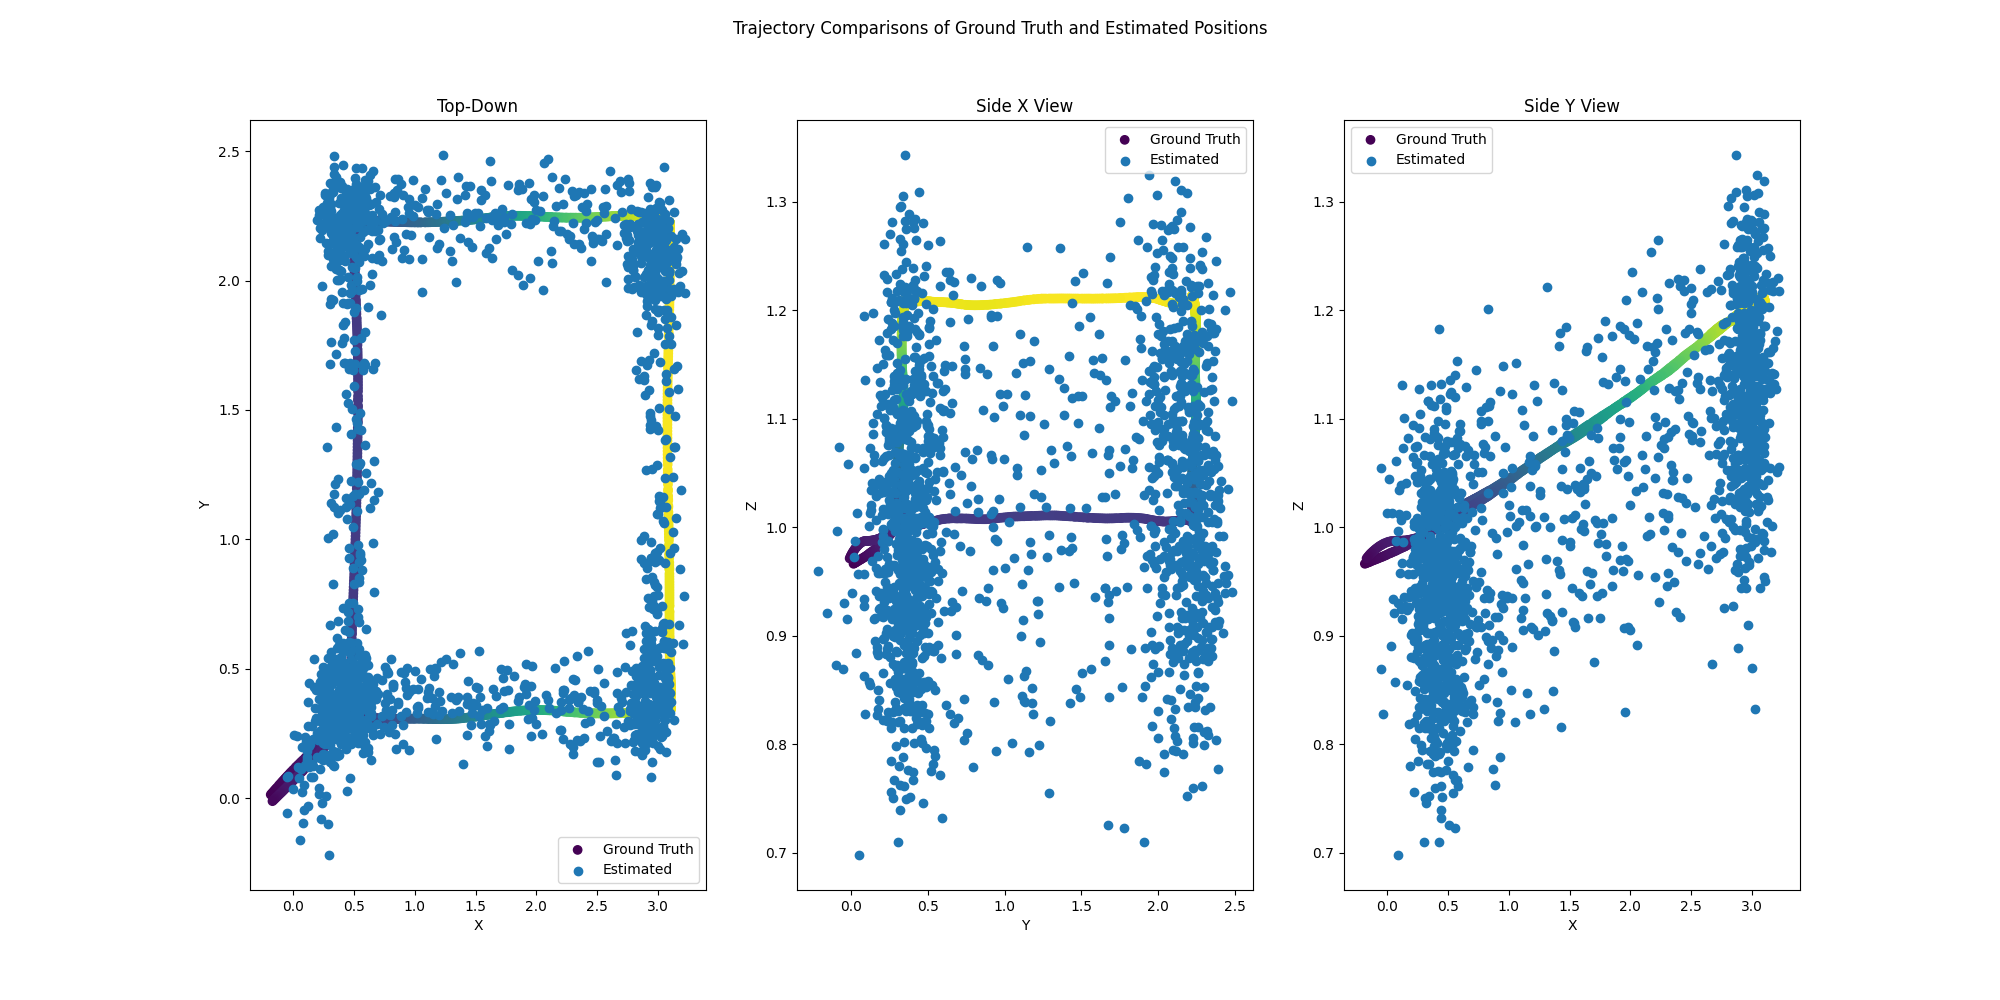
\includegraphics[width=0.8\textwidth]{./imgs/task1/studentdata5_positions.png}
    \caption{Dataset 5 Trajectories}
\end{figure}

\begin{figure}[H]
    \centering
    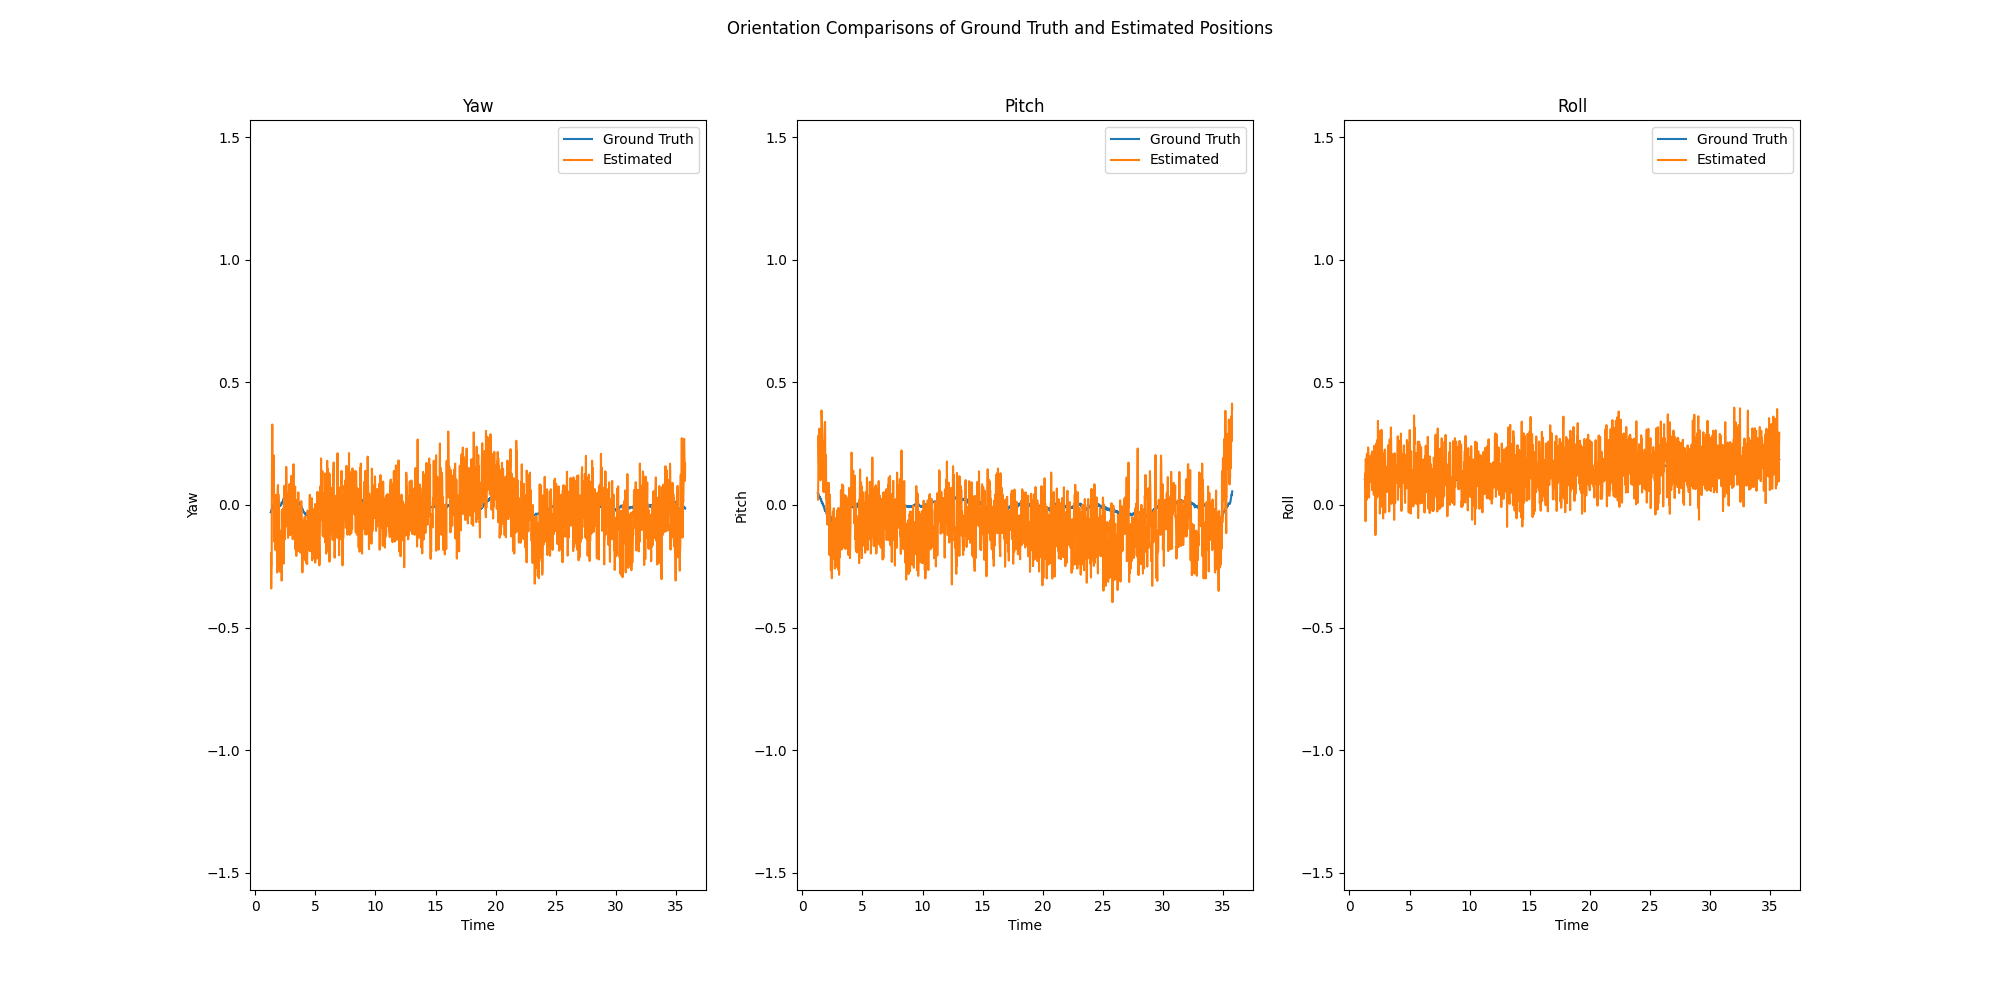
\includegraphics[width=0.8\textwidth]{./imgs/task1/studentdata5_orientations.png}
    \caption{Dataset 5 Orientations}
\end{figure}

\begin{figure}[H]
    \centering
    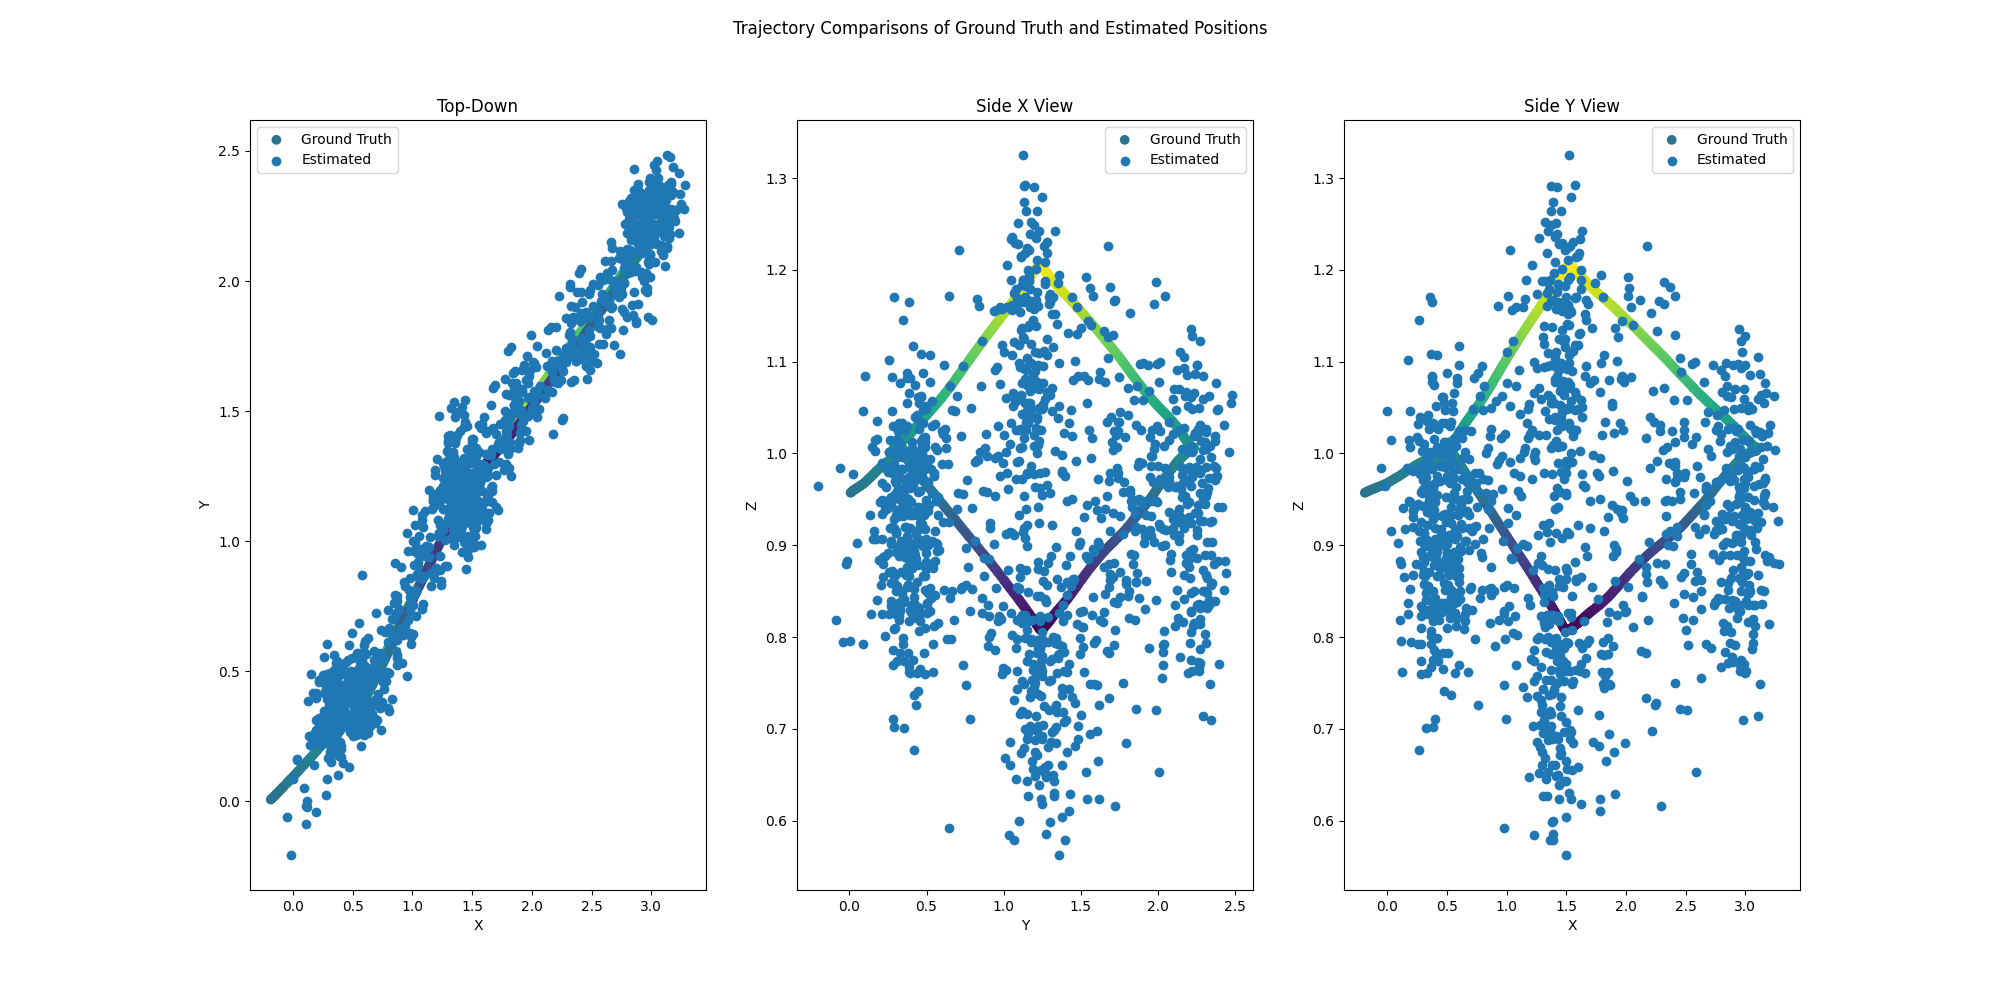
\includegraphics[width=0.8\textwidth]{./imgs/task1/studentdata6_positions.png}
    \caption{Dataset 6 Trajectories}
\end{figure}

\begin{figure}[H]
    \centering
    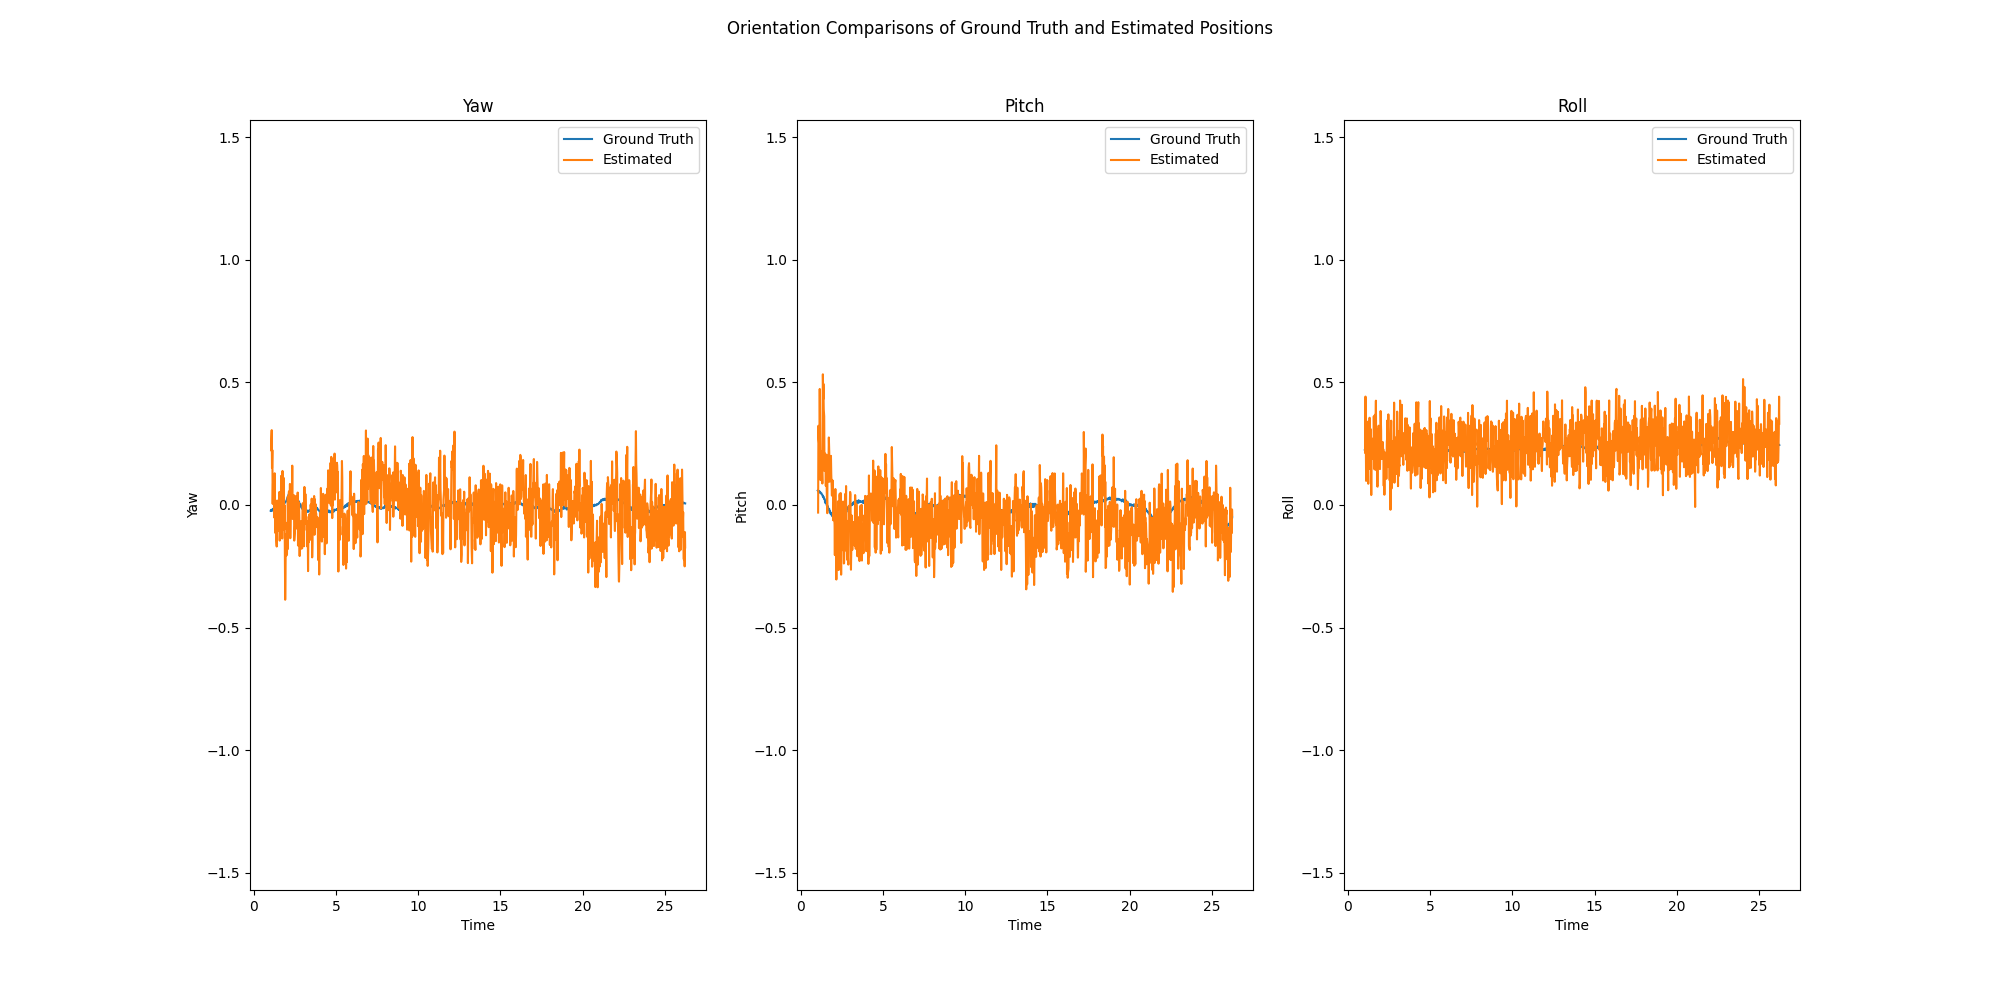
\includegraphics[width=0.8\textwidth]{./imgs/task1/studentdata6_orientations.png}
    \caption{Dataset 6 Orientations}
\end{figure}

\begin{figure}[H]
    \centering
    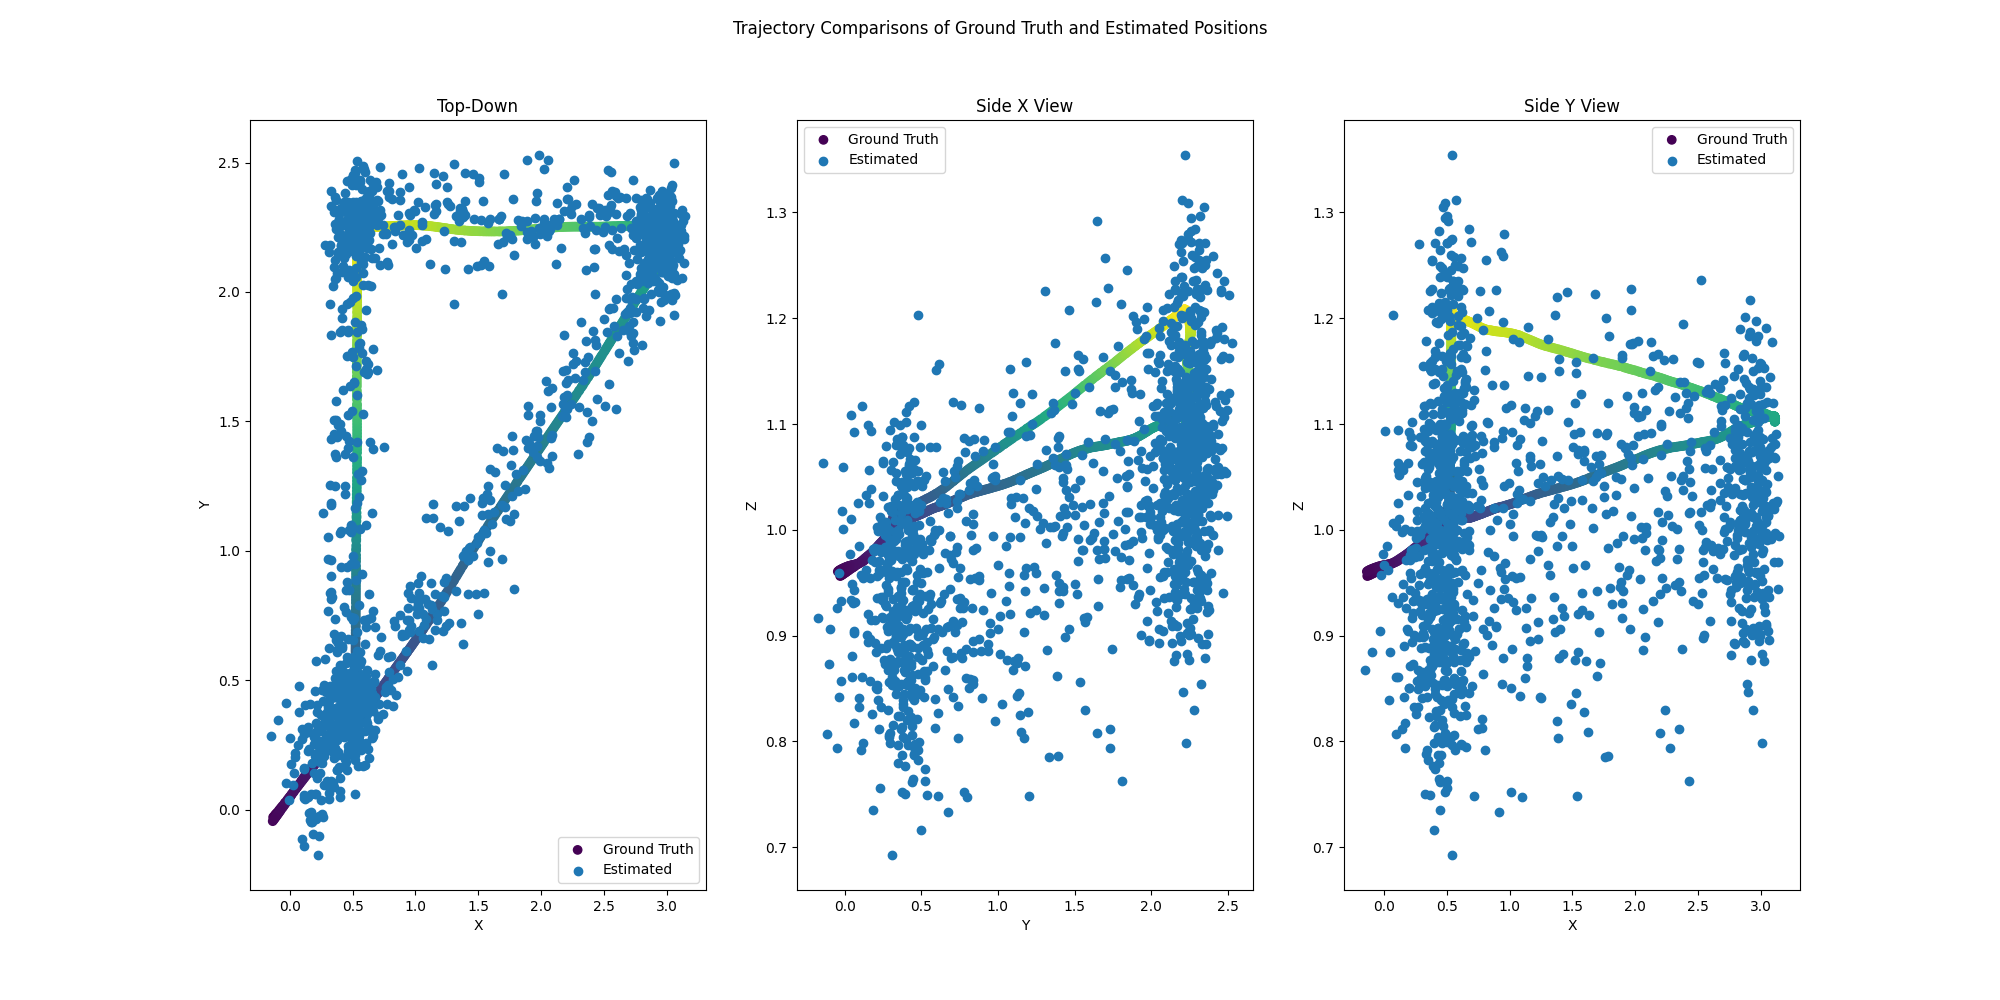
\includegraphics[width=0.8\textwidth]{./imgs/task1/studentdata7_positions.png}
    \caption{Dataset 7 Trajectories}
\end{figure}

\begin{figure}[H]
    \centering
    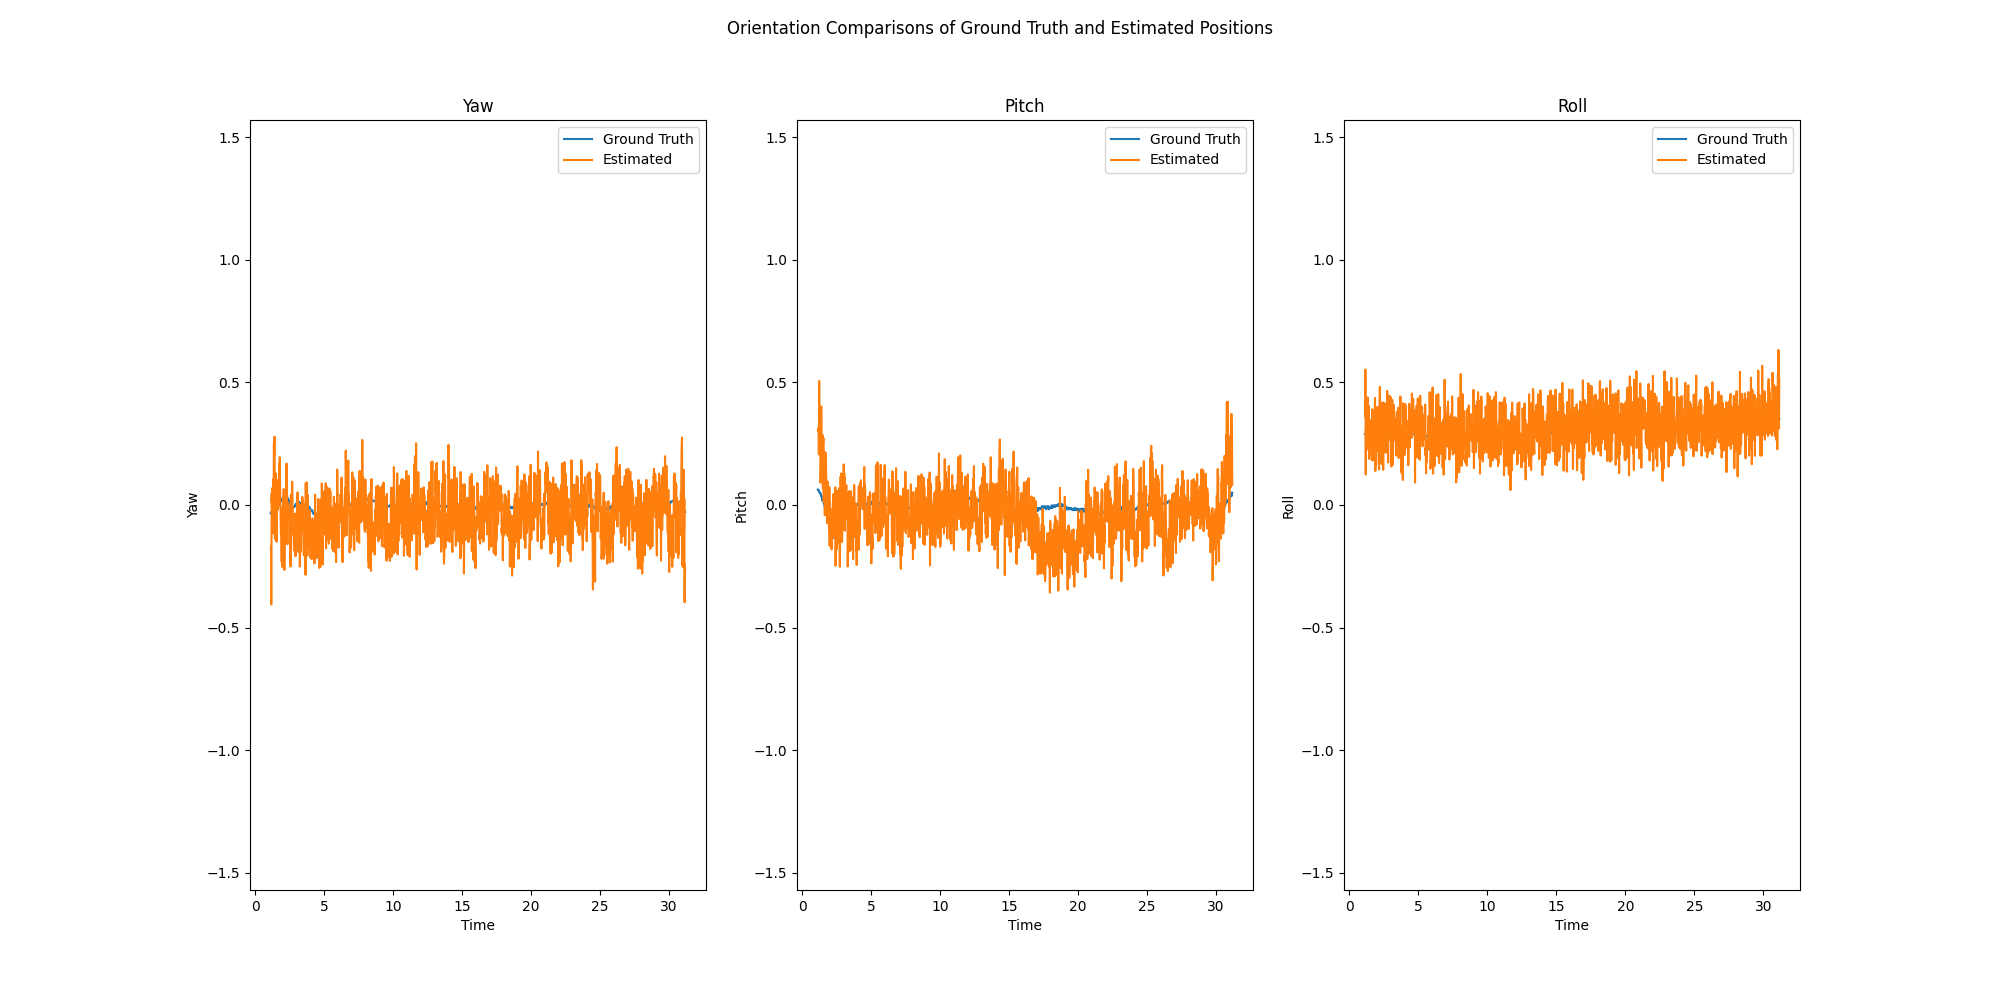
\includegraphics[width=0.8\textwidth]{./imgs/task1/studentdata7_orientations.png}
    \caption{Dataset 7 Orientations}
\end{figure}

\section*{Task 2}

In task 2 we are tasked with testing certain hyperparameters of our particle filter in order to observe performnace differences. Here we aim to test the sampling method - how we ascertain our estimate given our particles - and the effect of the number of particles on the performance of the filter.

\subsection*{Sampling Method}

First, we will explore the sampling method. We have three to test:

\begin{itemize}
    \item \textbf{Highest Weighted Particle} - We select the particle with the highest weight as our estimate.
    \item \textbf{Weighted Average} - We take the weighted average of all particles as our estimate.
    \item \textbf{Flat Average} - We take the flat average of all particles as our estimate, ignoring the weights.
\end{itemize}

This author predicted that weighted average would out perform the others. Below we have charts of the performance through RMSE of each dataset and method, with a steady $2000$ particles and unchanged parameters otherwise for each. We then show a table of average RMSE performance across datasets.

\begin{figure}[H]
    \centering
    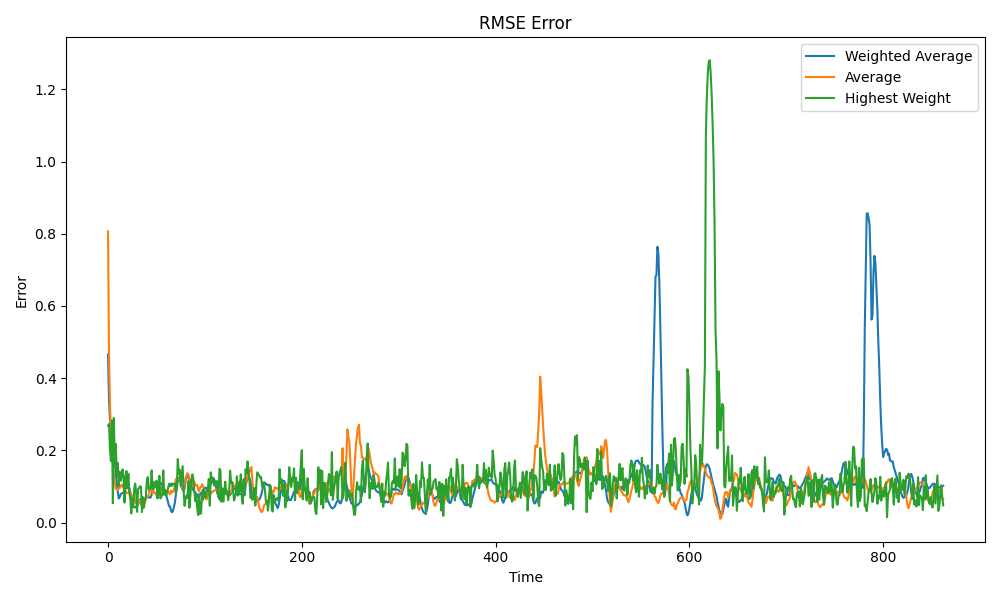
\includegraphics[width=0.8\textwidth]{./imgs/task2/studentdata1_rmse_methods.png}
    \caption{Dataset 1 Sampling Method Performance}
\end{figure}

\begin{figure}[H]
    \centering
    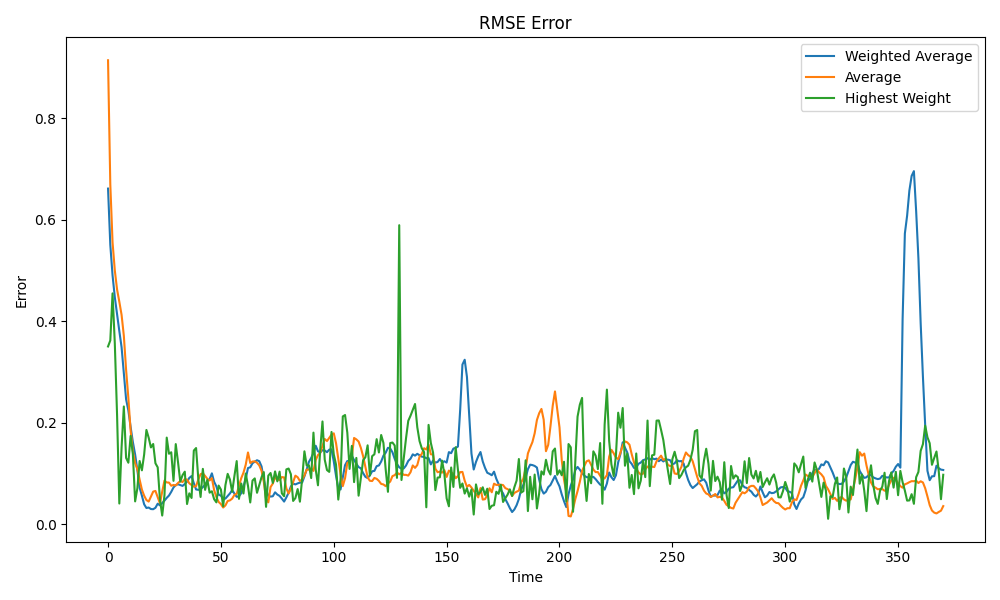
\includegraphics[width=0.8\textwidth]{./imgs/task2/studentdata2_rmse_methods.png}
    \caption{Dataset 2 Sampling Method Performance}
\end{figure}

\begin{figure}[H]
    \centering
    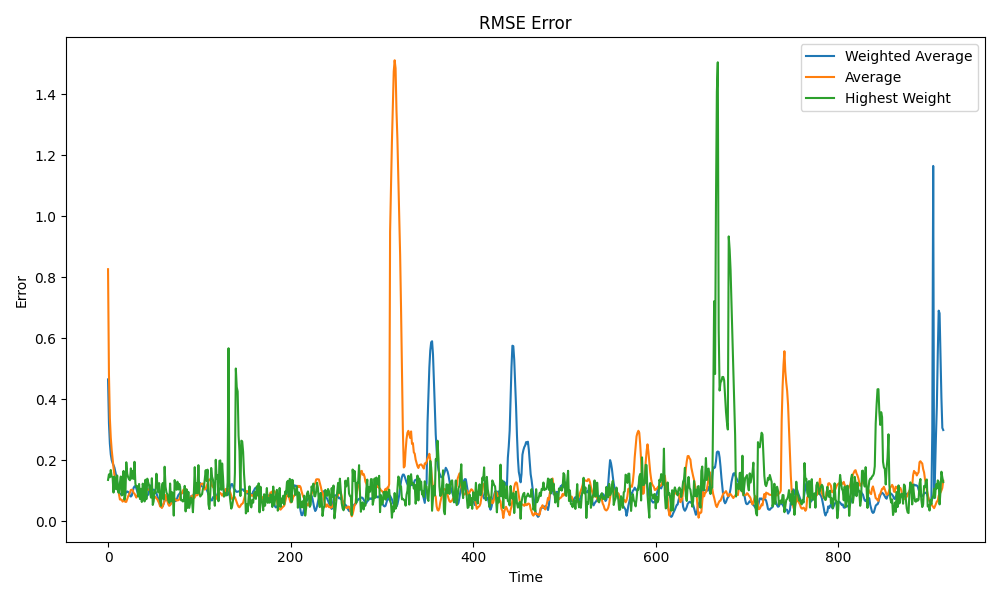
\includegraphics[width=0.8\textwidth]{./imgs/task2/studentdata3_rmse_methods.png}
    \caption{Dataset 3 Sampling Method Performance}
\end{figure}

\begin{figure}[H]
    \centering
    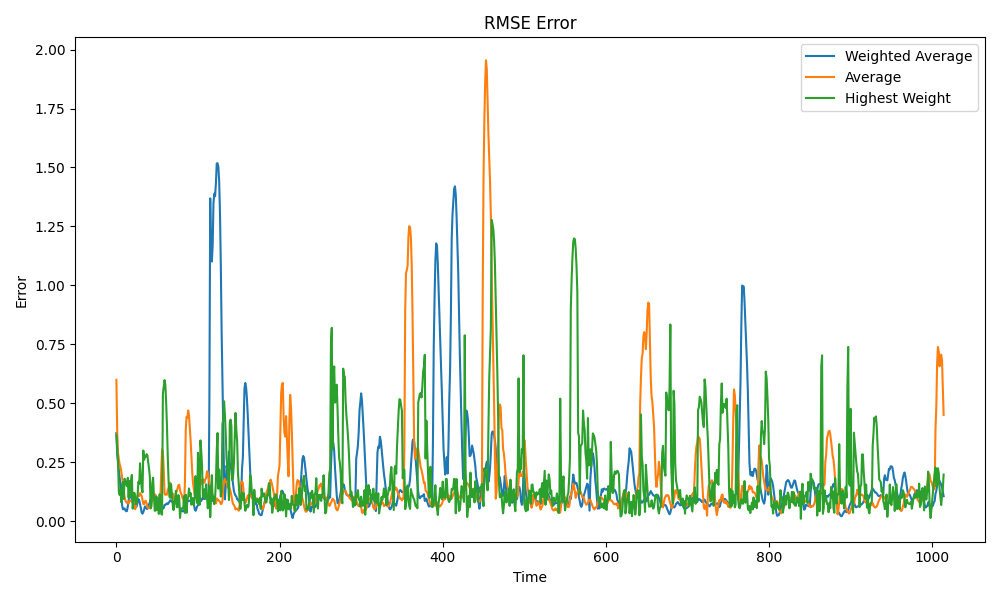
\includegraphics[width=0.8\textwidth]{./imgs/task2/studentdata4_rmse_methods.png}
    \caption{Dataset 4 Sampling Method Performance}
\end{figure}

\begin{figure}[H]
    \centering
    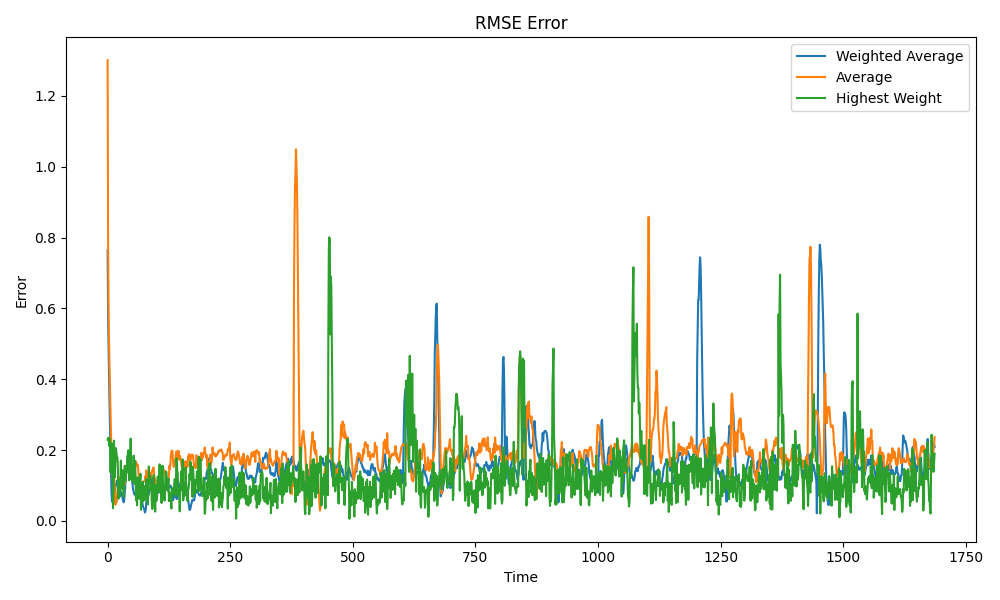
\includegraphics[width=0.8\textwidth]{./imgs/task2/studentdata5_rmse_methods.png}
    \caption{Dataset 5 Sampling Method Performance}
\end{figure}

\begin{figure}[H]
    \centering
    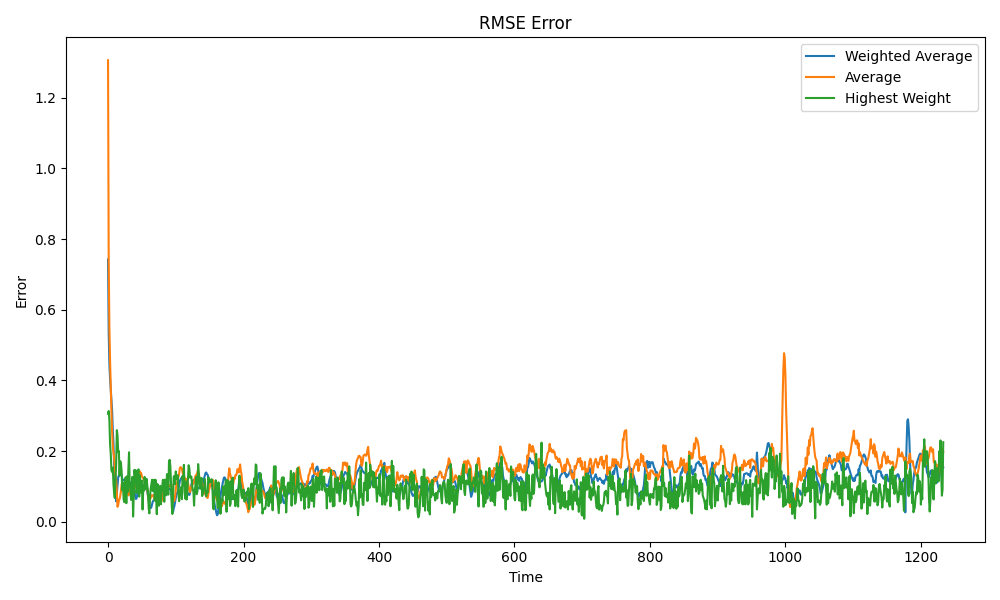
\includegraphics[width=0.8\textwidth]{./imgs/task2/studentdata6_rmse_methods.png}
    \caption{Dataset 6 Sampling Method Performance}
\end{figure}

\begin{figure}[H]
    \centering
    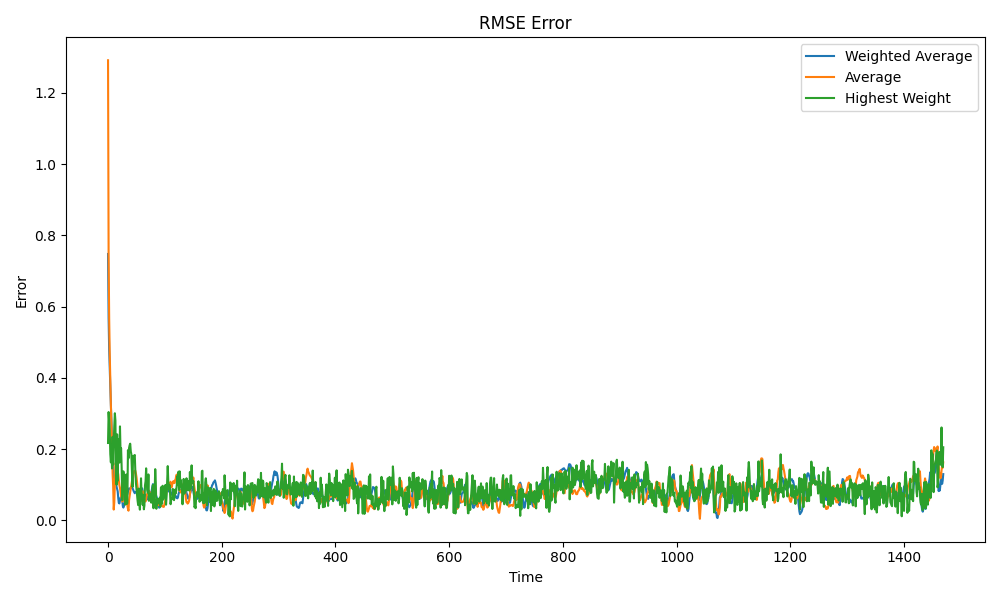
\includegraphics[width=0.8\textwidth]{./imgs/task2/studentdata7_rmse_methods.png}
    \caption{Dataset 7 Sampling Method Performance}
\end{figure}

And our performance numerically presented:

\begin{table}[H]
    \centering
    \begin{tabular}{|c|c|c|c|}
        \hline
        \textbf{Dataset} & \textbf{Weighted Average} & \textbf{Averaged} & \textbf{Highest Weighted Particle} \\ \hline
        0                & nan                       & 1767.595          & 2070.701                           \\ \hline
        1                & 0.113                     & 0.100             & 0.121                              \\ \hline
        2                & 0.117                     & 0.103             & 0.108                              \\ \hline
        3                & 0.100                     & 0.117             & 0.117                              \\ \hline
        4                & 0.175                     & 0.170             & 0.183                              \\ \hline
        5                & 0.156                     & 0.192             & 0.127                              \\ \hline
        6                & 0.120                     & 0.147             & 0.093                              \\ \hline
        7                & 0.084                     & 0.083             & 0.088                              \\ \hline
    \end{tabular}
\end{table}

Again, \textit{studentdata0} is notably poor performance due to the camera losing sight of the AprilTags. We could get good performance from this dataset, but it required significantly higher noise. Since we are aiming to not tune the filter to a specific dataset, we keep the best performing across all other datasets.

To this author's surprised, the highest weighted particle often outperformed the other methods. That being said, it does seem to be slightly less "smoothed" in the charts, showing that it may present better results overall but has a higher likelihood of suffering from poor measurements.

For the remainder of this assignment, the highest weighted particle method will be used unless otherwise stated.

\subsection*{Particle Count}

Now we seek to determine the effect of particle counts on the datasets. We are looking at the performance of $250$, $500$, $750$, $1000$, $2000$, $3000$, $4000$, and $5000$ particles.

\begin{figure}[H]
    \centering
    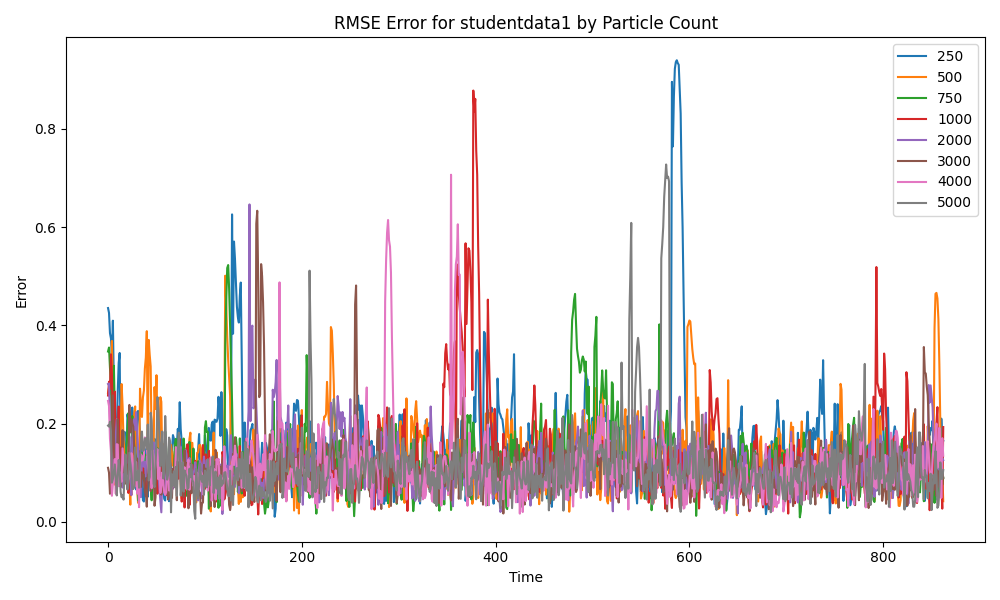
\includegraphics[width=0.8\textwidth]{./imgs/task2/studentdata1_rmse_particle_count.png}
    \caption{Dataset 1 Particle Count Performance}
\end{figure}

\begin{figure}[H]
    \centering
    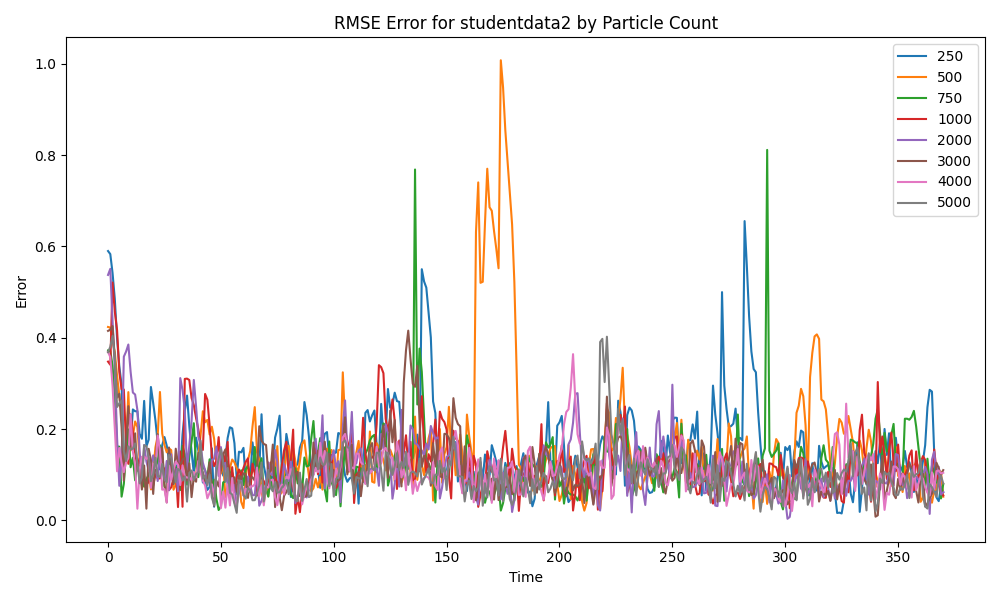
\includegraphics[width=0.8\textwidth]{./imgs/task2/studentdata2_rmse_particle_count.png}
    \caption{Dataset 2 Particle Count Performance}
\end{figure}

\begin{figure}[H]
    \centering
    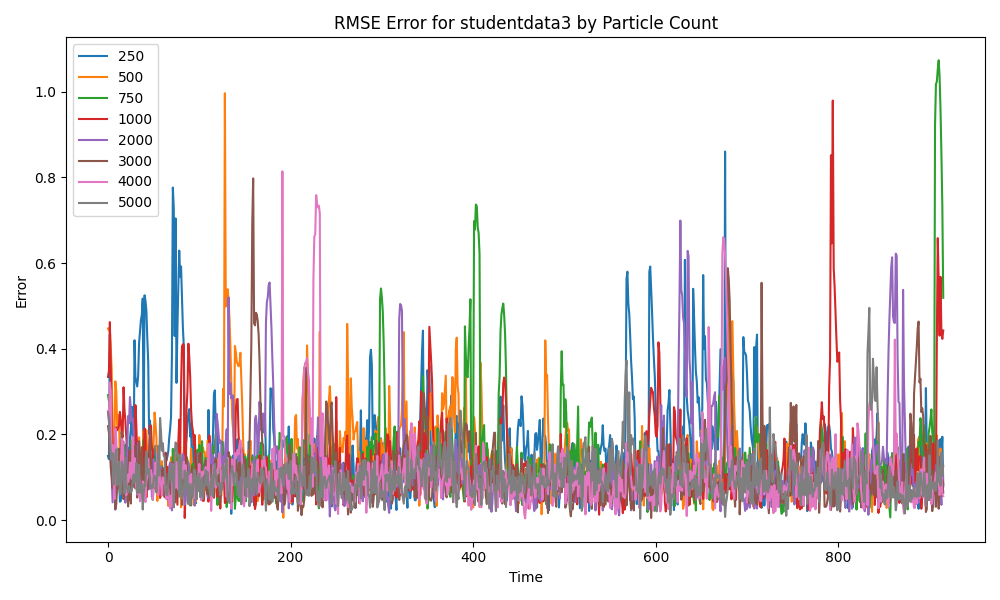
\includegraphics[width=0.8\textwidth]{./imgs/task2/studentdata3_rmse_particle_count.png}
    \caption{Dataset 3 Particle Count Performance}
\end{figure}

\begin{figure}[H]
    \centering
    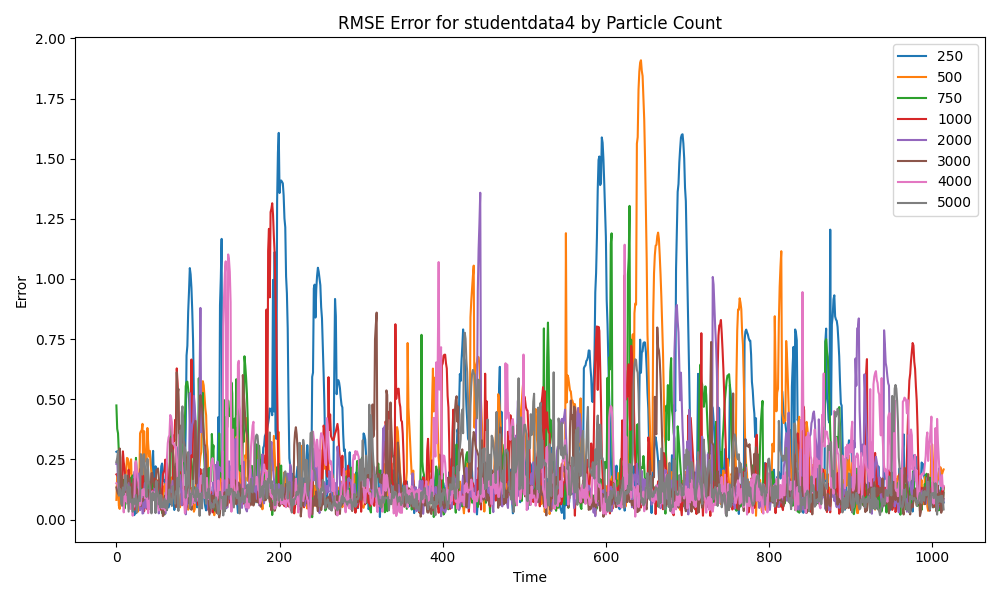
\includegraphics[width=0.8\textwidth]{./imgs/task2/studentdata4_rmse_particle_count.png}
    \caption{Dataset 4 Particle Count Performance}
\end{figure}

\begin{figure}[H]
    \centering
    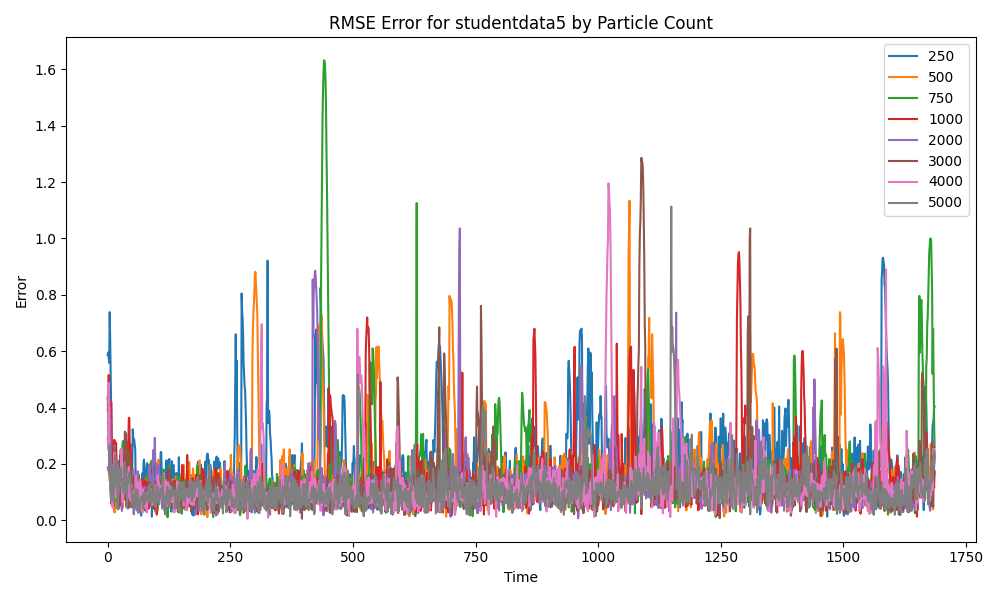
\includegraphics[width=0.8\textwidth]{./imgs/task2/studentdata5_rmse_particle_count.png}
    \caption{Dataset 5 Particle Count Performance}
\end{figure}

\begin{figure}[H]
    \centering
    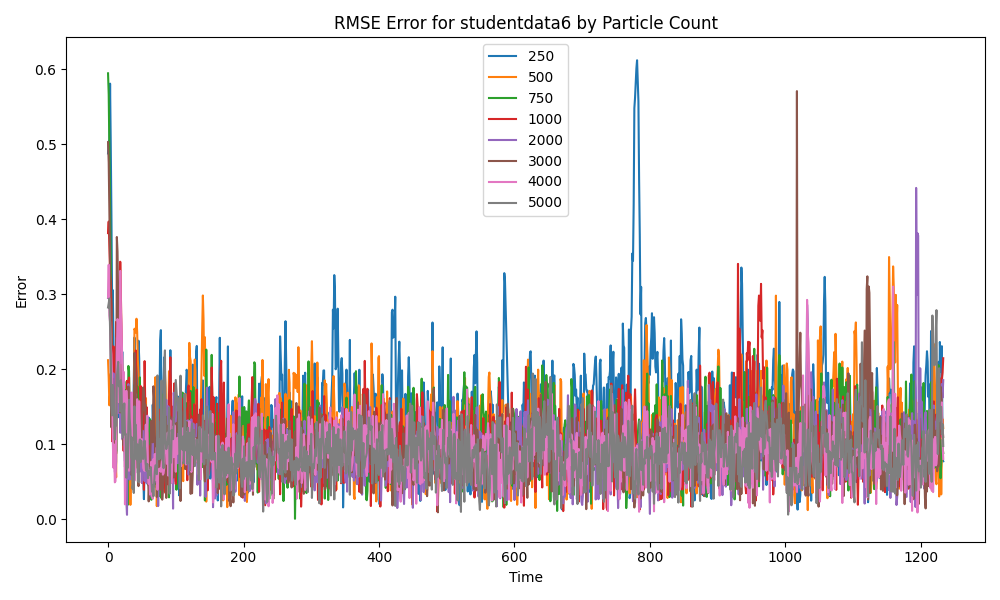
\includegraphics[width=0.8\textwidth]{./imgs/task2/studentdata6_rmse_particle_count.png}
    \caption{Dataset 6 Particle Count Performance}
\end{figure}

\begin{figure}[H]
    \centering
    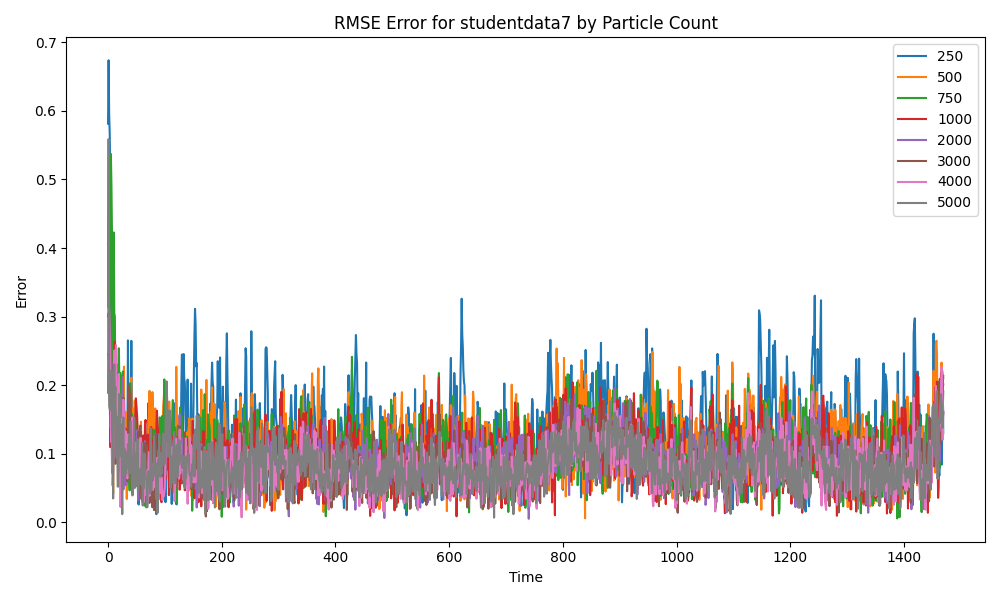
\includegraphics[width=0.8\textwidth]{./imgs/task2/studentdata7_rmse_particle_count.png}
    \caption{Dataset 7 Particle Count Performance}
\end{figure}

And our performance numerically presented to make do for the otherwise crowded charts:

\begin{table}[H]
    \centering
    \begin{tabular}{|c|c|c|c|c|c|c|c|c|c|}
        \hline
        \textbf{Particles} & \textbf{250} & \textbf{500} & \textbf{750} & \textbf{1000} & \textbf{2000} & \textbf{3000} & \textbf{4000} & \textbf{5000} \\ \hline
        \textbf{Dataset 1} & 0.169        & 0.145        & 0.139        & 0.112         & 0.108         & 0.110         & 0.111         & 0.114         \\ \hline
        \textbf{Dataset 2} & 0.192        & 0.159        & 0.131        & 0.125         & 0.118         & 0.104         & 0.111         & 0.107         \\ \hline
        \textbf{Dataset 3} & 0.187        & 0.143        & 0.146        & 0.134         & 0.119         & 0.106         & 0.102         & 0.096         \\ \hline
        \textbf{Dataset 4} & 0.239        & 0.204        & 0.186        & 0.209         & 0.151         & 0.152         & 0.149         & 0.157         \\ \hline
        \textbf{Dataset 5} & 0.197        & 0.159        & 0.152        & 0.149         & 0.142         & 0.133         & 0.113         & 0.122         \\ \hline
        \textbf{Dataset 6} & 0.140        & 0.110        & 0.114        & 0.105         & 0.094         & 0.091         & 0.093         & 0.089         \\ \hline
        \textbf{Dataset 7} & 0.132        & 0.109        & 0.102        & 0.097         & 0.089         & 0.085         & 0.085         & 0.083         \\ \hline
        \textbf{Average}   & 0.175        & 0.147        & 0.134        & 0.129         & 0.116         & 0.110         & 0.113         & 0.108         \\ \hline
    \end{tabular}
\end{table}

Here we clearly see that performance does improve with more particles - but this is only half the store. We also recorded time to perform across the entire dataset to demonstrate the effect increasing the particle count has on processing time:

\begin{table}[H]
    \centering
    \begin{tabular}{|c|c|c|c|c|c|c|c|c|c|}
        \hline
        \textbf{Particles} & \textbf{250} & \textbf{500} & \textbf{750} & \textbf{1000} & \textbf{2000} & \textbf{3000} & \textbf{4000} & \textbf{5000} \\ \hline
        \textbf{Dataset 1} & 4.39         & 8.04         & 12.69        & 16.81         & 27.85         & 45.15         & 57.45         & 68.63         \\ \hline
        \textbf{Dataset 2} & 2.18         & 3.84         & 5.08         & 6.23          & 12.17         & 19.01         & 25.67         & 28.69         \\ \hline
        \textbf{Dataset 3} & 5.24         & 9.29         & 13.15        & 16.96         & 31.00         & 46.10         & 59.97         & 73.82         \\ \hline
        \textbf{Dataset 4} & 4.92         & 8.77         & 12.97        & 18.31         & 35.33         & 49.52         & 65.80         & 81.54         \\ \hline
        \textbf{Dataset 5} & 8.62         & 16.04        & 21.19        & 29.19         & 55.45         & 84.19         & 107.83        & 138.57        \\ \hline
        \textbf{Dataset 6} & 5.80         & 10.67        & 16.80        & 21.37         & 39.68         & 61.62         & 78.87         & 103.59        \\ \hline
        \textbf{Dataset 7} & 8.22         & 14.92        & 21.13        & 24.46         & 53.17         & 74.71         & 98.45         & 123.14        \\ \hline
    \end{tabular}
\end{table}

Here we see, in seconds, the dramatically increasing time to process the datasets as particle counts increase. Further optimization of the code - such as fixing the few non vectorized operations, or abandoning Python entirely for an actually performant language, could help alleviate this. This is a crucial consideration for a particle filter - if the filter is expected to run in real time, we must consider the time performance of its calculations.

For the remainder of this assignment, we will utilize $2000$ particles unless specified.


\section*{Task 3}

In this section, we are tasked with comparing with the nonlinear Kalman filter produced in our prior assignment - for this author, a UKF filter. The filter has been ported into \textbf{ukf.py} and is not heavily changed from the prior assignment.

For this, we ran the UKF filter against the 2000 and 5000 particle filter runs utilizing the highest weighted particle method. We then compared the RMSE of the UKF filter against the particle filter.

\begin{figure}[H]
    \centering
    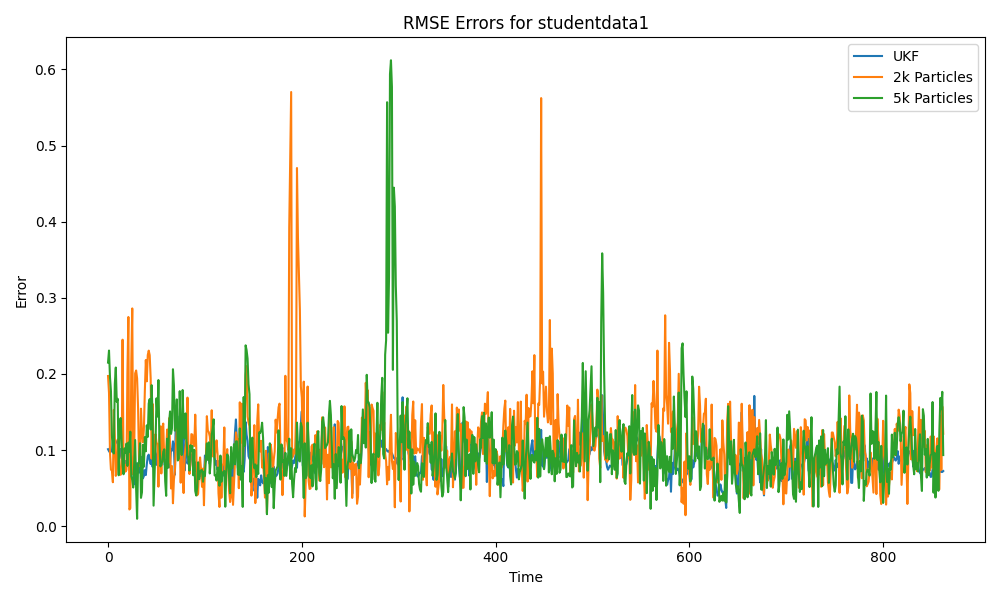
\includegraphics[width=0.8\textwidth]{./imgs/task3/studentdata1_rmse.png}
    \caption{Dataset 1 RMSE Comparison}
\end{figure}

\begin{figure}[H]
    \centering
    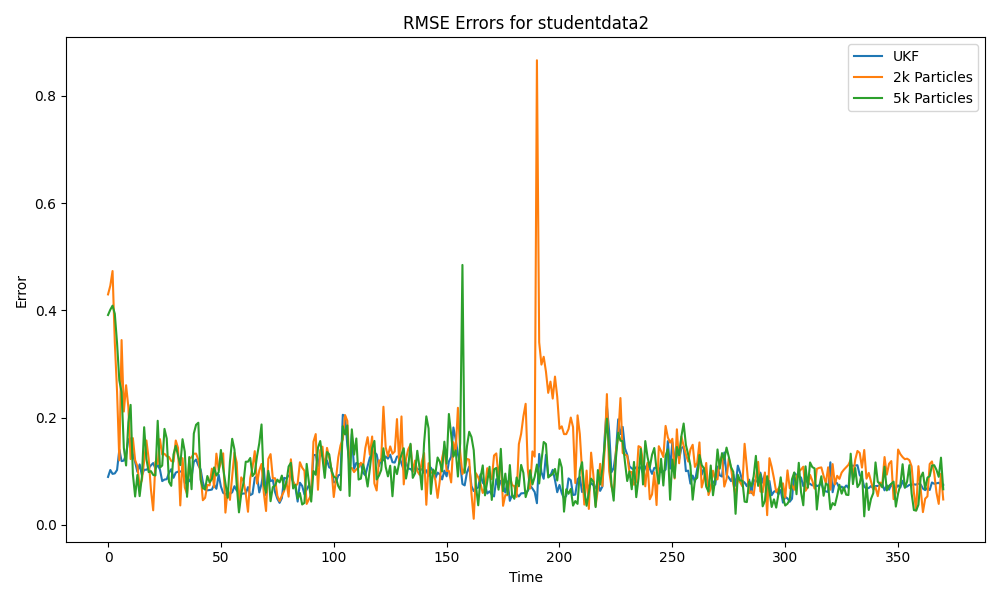
\includegraphics[width=0.8\textwidth]{./imgs/task3/studentdata2_rmse.png}
    \caption{Dataset 2 RMSE Comparison}
\end{figure}

\begin{figure}[H]
    \centering
    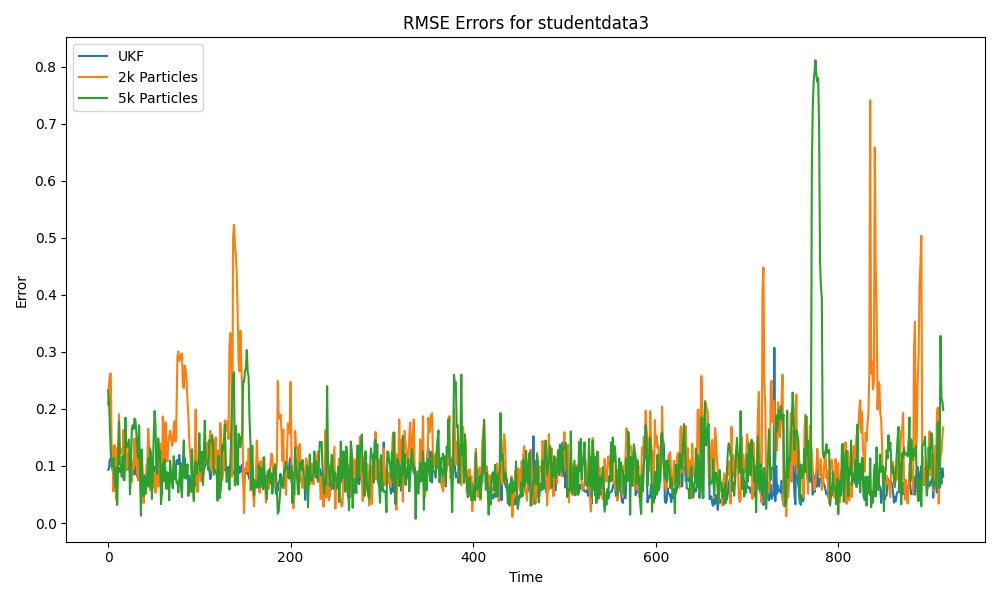
\includegraphics[width=0.8\textwidth]{./imgs/task3/studentdata3_rmse.png}
    \caption{Dataset 3 RMSE Comparison}
\end{figure}

\begin{figure}[H]
    \centering
    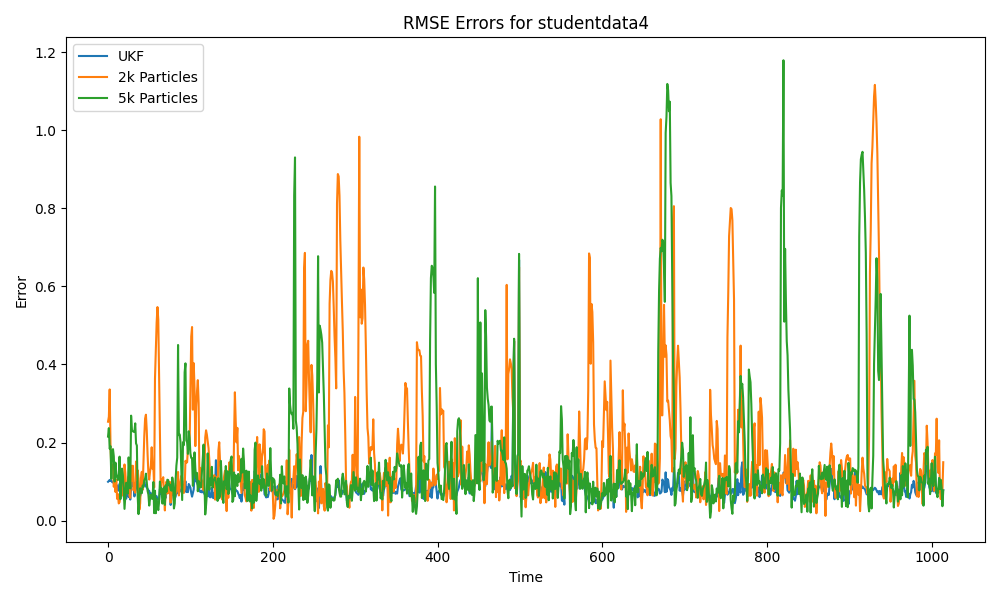
\includegraphics[width=0.8\textwidth]{./imgs/task3/studentdata4_rmse.png}
    \caption{Dataset 4 RMSE Comparison}
\end{figure}

\begin{figure}[H]
    \centering
    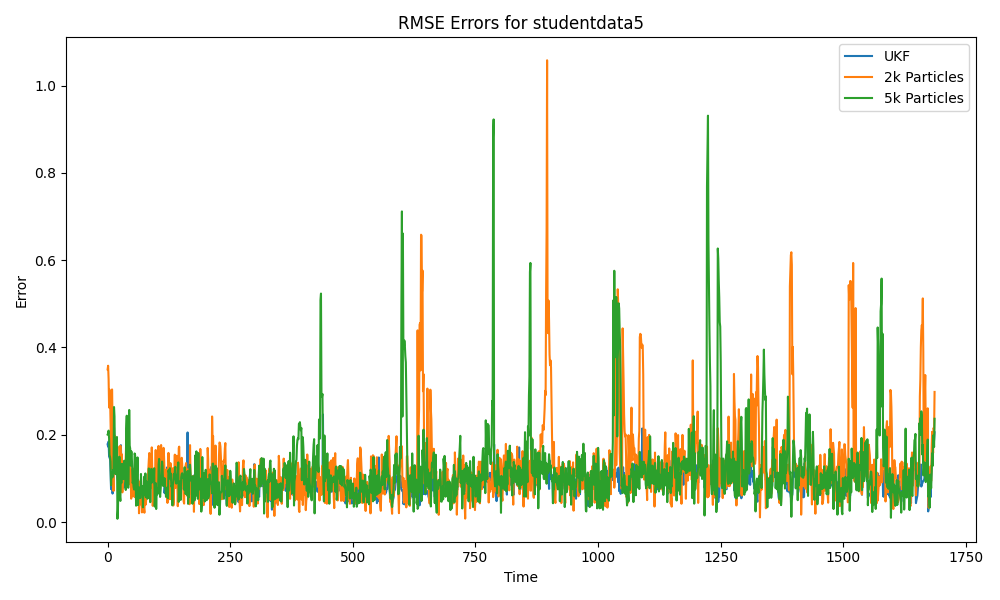
\includegraphics[width=0.8\textwidth]{./imgs/task3/studentdata5_rmse.png}
    \caption{Dataset 5 RMSE Comparison}
\end{figure}

\begin{figure}[H]
    \centering
    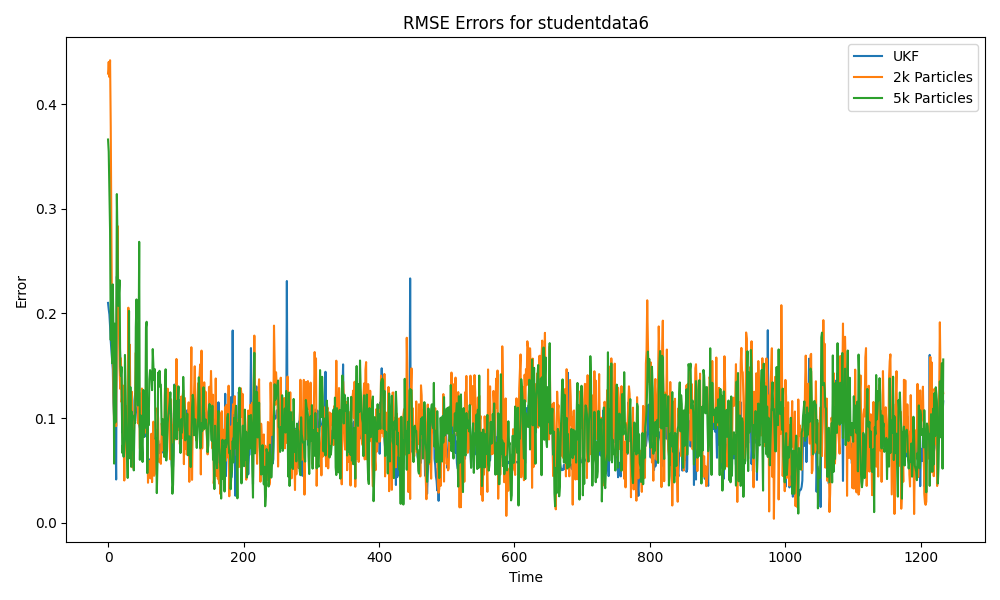
\includegraphics[width=0.8\textwidth]{./imgs/task3/studentdata6_rmse.png}
    \caption{Dataset 6 RMSE Comparison}
\end{figure}

\begin{figure}[H]
    \centering
    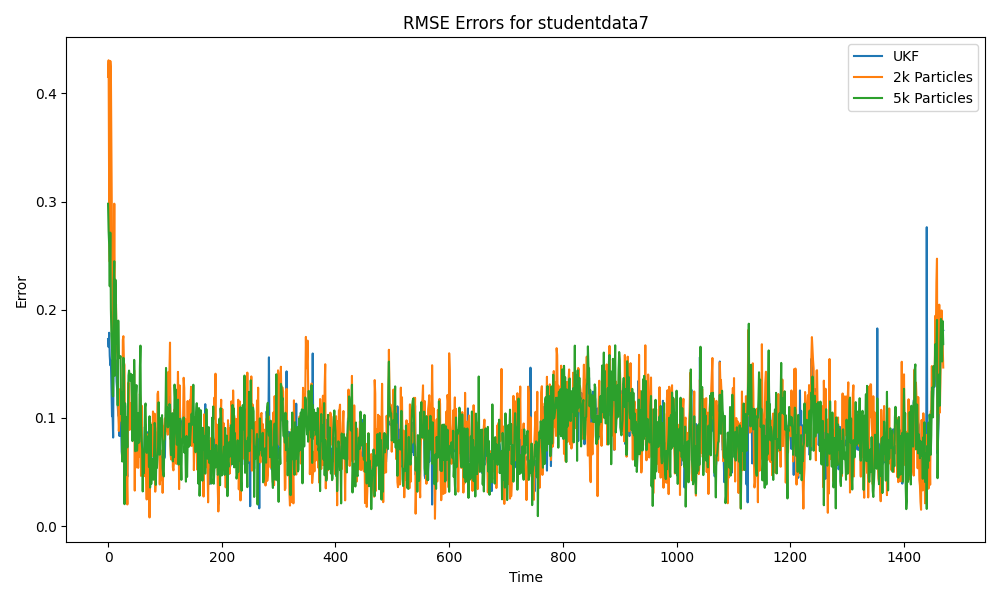
\includegraphics[width=0.8\textwidth]{./imgs/task3/studentdata7_rmse.png}
    \caption{Dataset 7 RMSE Comparison}
\end{figure}

And our table of RMSE performance:

\begin{table}[H]
    \centering
    \begin{tabular}{|c|c|c|c|}
        \hline
        \textbf{Dataset} & \textbf{UKF} & \textbf{2k} & \textbf{5k} \\ \hline
        \textbf{1}       & 0.087        & 0.109       & 0.102       \\ \hline
        \textbf{2}       & 0.091        & 0.116       & 0.103       \\ \hline
        \textbf{3}       & 0.076        & 0.115       & 0.105       \\ \hline
        \textbf{4}       & 0.084        & 0.175       & 0.153       \\ \hline
        \textbf{5}       & 0.090        & 0.125       & 0.119       \\ \hline
        \textbf{6}       & 0.080        & 0.094       & 0.090       \\ \hline
        \textbf{7}       & 0.082        & 0.088       & 0.084       \\ \hline
        \textbf{Average} & 0.084        & 0.116       & 0.107       \\ \hline
    \end{tabular}
\end{table}

Here we see that UKF does out perform our particle filter, but with the trending downwards error as particles increase, it is likely that more particles would outperform the UKF filter.

Notable, however, is the execution time of the UKf filter versus the particle filter- it takes a few seconds - averaging $3.2$ seconds across datasets - to complete a full dataset; an order of magnitude less than the 2000 particle filter, which in turn is twice as quick as the 5000 particle filter.

So when do we utilize one, or the other? First, we consider our state model and target - is it a highly nonlinear system? The greater the nonlinearity, the more likely that UKF will not be able to deal with the system. The particle filter is more resilient to this, and will be a more accurate filter in such a problem.

The next consideration is the time to process - if we are in a system with limited compute and a hard requirement for a high speed filter, we may not be able to utilize a particle filter. While compute continues to increase while size, power consumption, and cost continue to decrease, the number of particles required for a particle filter to perform in a given state space grows dramatically as you expand the state space. Thus a high dimensional state space problem may be computationally prohibitive even on modern hardware, denoting preference towards the UKF.

That being said, this author believes the particle filter was significantly easier to code for, as it did not require significant mathematical understanding or modeling of the system in order to implement. Similarly, the randomness of the particle filter led to much less tuning than our time with UKF, as it was robust through its randomness to the system's noise.



\end{document}